%\documentclass[compress]{beamer}

\documentclass[13.5pt]{beamer}
\usetheme{default} 
%\usetheme{Warsaw}

\usepackage{etex}
\usepackage{makeidx}  % allows for indexgeneration
\usepackage{mathtools} %
\usepackage{booktabs} %
\usepackage{verbatim} %
\usepackage{graphicx} %
\usepackage[labelformat=empty]{caption}
%\usepackage{caption}
%\usepackage{subcaption}
%\usepackage{hyperref}
%\usepackage{subfigure} %
\usepackage{amsmath}
\usepackage{amssymb}
\usepackage{amsthm}
\usepackage{xspace}
\usepackage{natbib}
%\usepackage{subfigure} %
\usepackage{pifont}%
\usepackage{tikz}
\usepackage{relsize}
\usepackage{multirow}
\usepackage{slashbox}
\usepackage{textcomp}
\usepackage{comment}
\usepackage{url}
\usepackage{float}
\usepackage{algorithmic} 
% \usepackage{algpseudocode} 
%\usepackage{algorithm}
\usepackage[vlined]{algorithm2e} 

\usepackage{subfig}
\usepackage{framed}
\usepackage{empheq}
\usepackage{caption}

\newcommand{\cmark}{\ding{51}}%
\newcommand{\xmark}{\ding{55}}%
\newcommand{\vectornorm}[1]{\left|\left|#1\right|\right|}
\newcommand{\argmin}{\operatornamewithlimits{argmin}}
\newcommand{\argmax}{\operatornamewithlimits{argmax}}


\author{{\Large} \\ 
\vspace{2.5cm}

\includegraphics[width=2.0cm]{cmulogo.jpeg}}

\title{{\bf \huge Time-course Gene expression Analysis}}

\begin{document}

\date{}

\frame{\titlepage}

\begin{frame}
\frametitle{Selected Time Points}

\begin{itemize}
\item Selected $15$ time points from mRNA is:
\[0.5, 1.0, 1.5, 2.5, 3.0, 4.5, 6.0, 7.5, 8.5, 9.5, 10.0, 12.5, 18.0, 24.0, 28.0\]
%\vspace{0.1cm}
\item Top $10$ solutions are similar to these selected points
\end{itemize}

\vspace{0.4cm}

\begin{itemize}
\item Initialize by points that sorted by increasing absolute differences.
\vspace{0.1cm}
\item Keep adding and removing points until there is no improvement.
\end{itemize}

\end{frame}


\begin{frame}
\frametitle{Error By Increasing Sampled Points}

\begin{itemize}
\item Major performance improvement over randomly selected points
\end{itemize}

\begin{figure}[h]
\begin{minipage}{1.0\textwidth}
\subfloat[Performance analysis]{\includegraphics[scale=0.15]{{../newdata/perform}.png}}
\hfill
\subfloat[Remove last two points]{\includegraphics[scale=0.15]{{../newdata/performRL2}.png}}
\end{minipage}
\label{fig:errplots}
\end{figure}

\end{frame}


\begin{frame}
\frametitle{mRNA Cluster Analysis}

\begin{itemize}
\item $6$ stable clusters
\begin{itemize}
\item One cluster corresponds to the genes with non-monotonic expression
  over time
\end{itemize}
\end{itemize}

\begin{figure}[h]
\begin{minipage}{1.0\textwidth}
\subfloat[6 stable clusters]{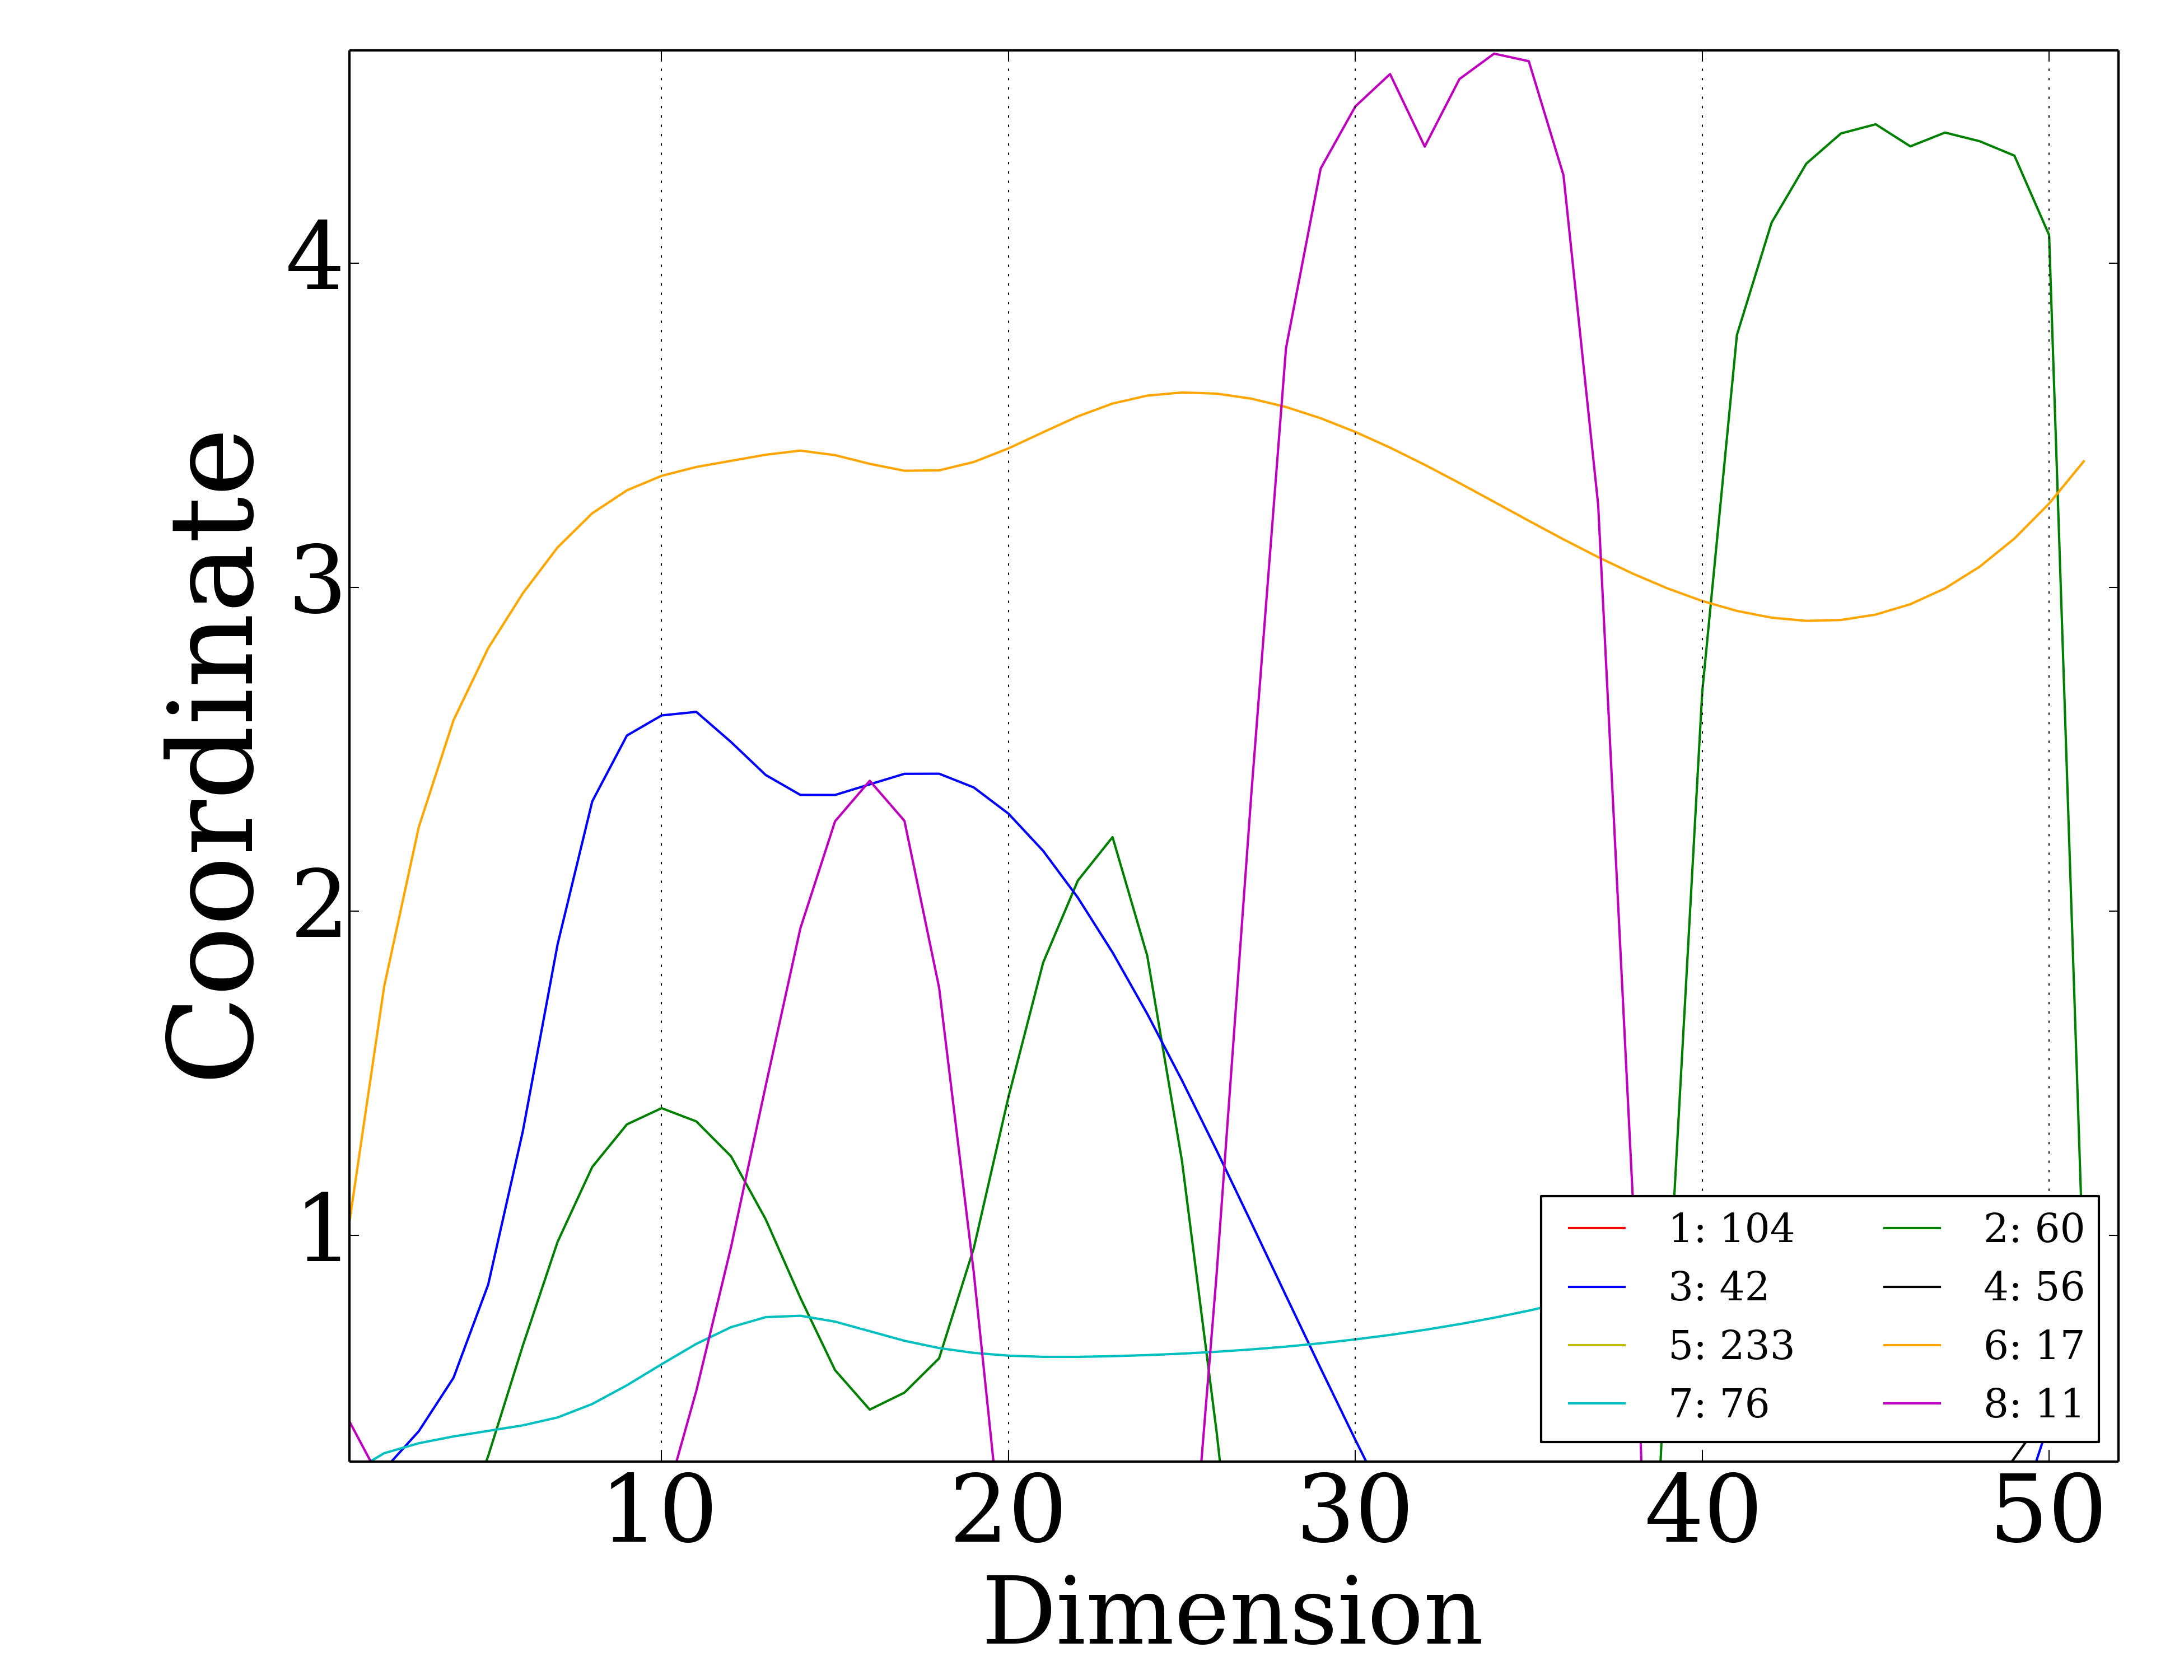
\includegraphics[scale=0.15]{{../newdata/centplotlimit}.png}}
\hfill
\subfloat[Centroids]{\includegraphics[scale=0.15]{{../newdata/centplot}.png}}
\end{minipage}
\label{fig:centplots}
\end{figure}

\end{frame}


\begin{frame}
\frametitle{Detailed mRNA Gene Analysis}

\begin{figure}[h]
\begin{minipage}{1.0\textwidth}
\subfloat[PDGFRA]{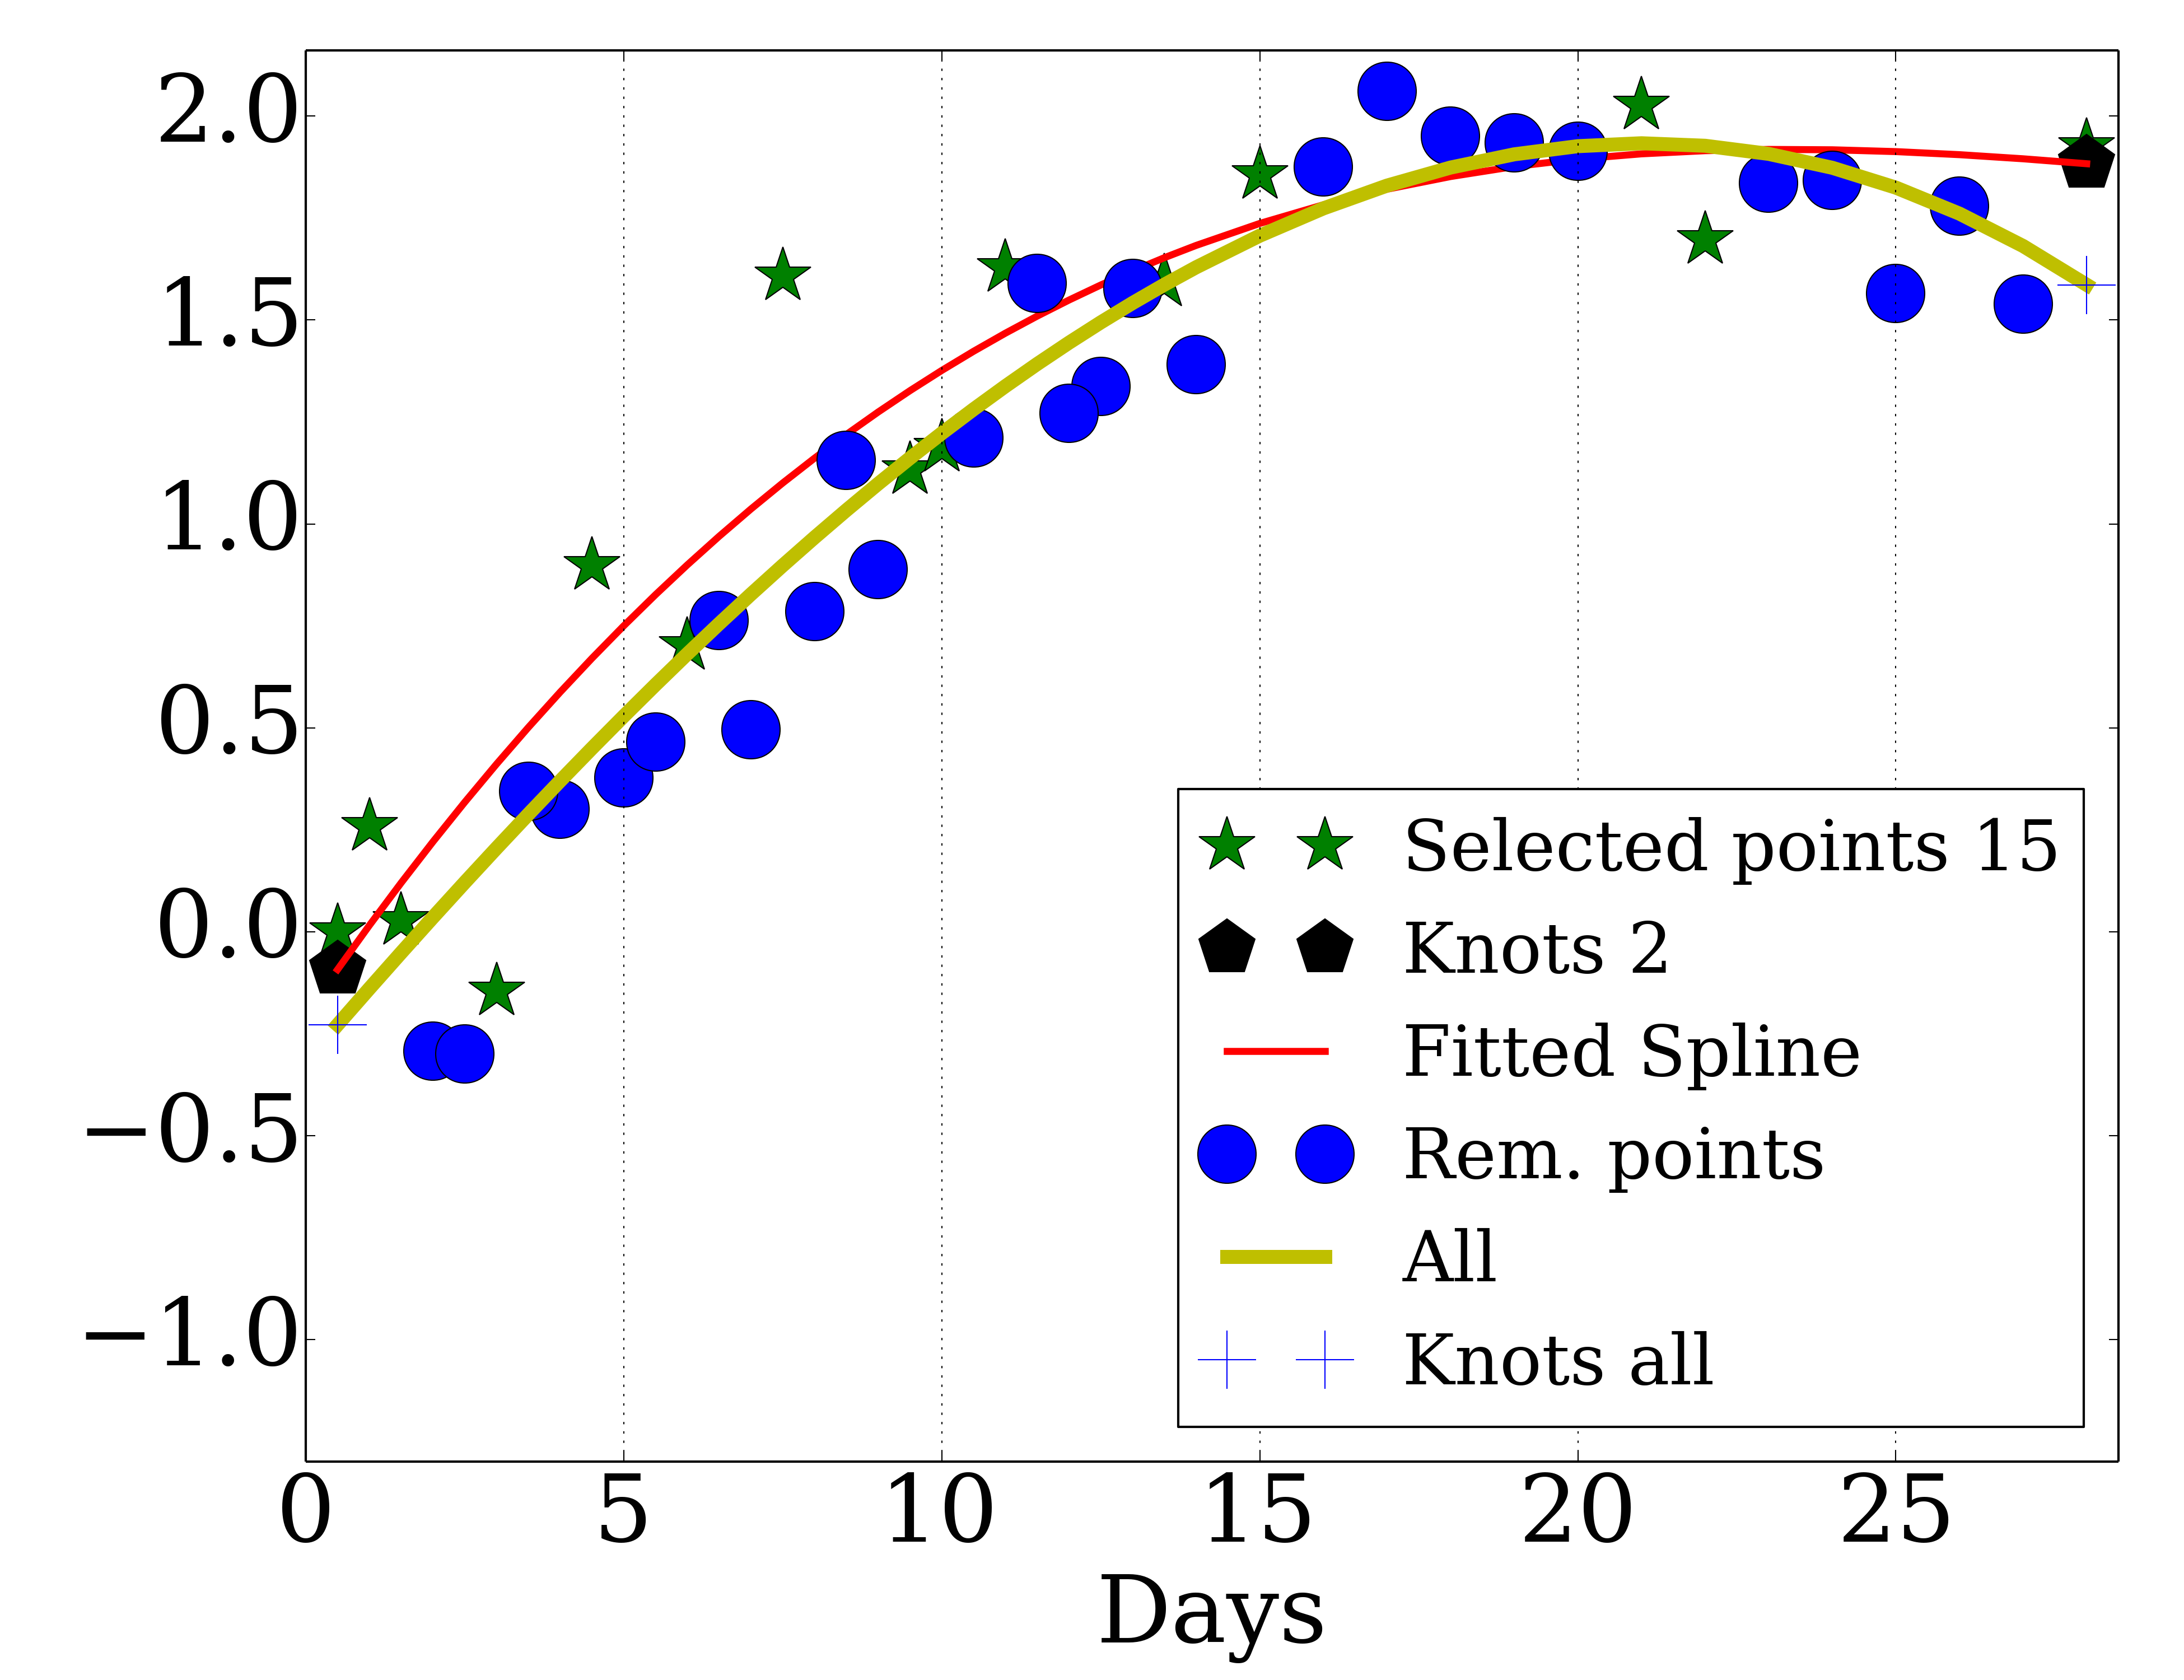
\includegraphics[scale=0.12]{{../newdata/PDGFRA_15_all}.png}}
\hfill
\subfloat[ELN]{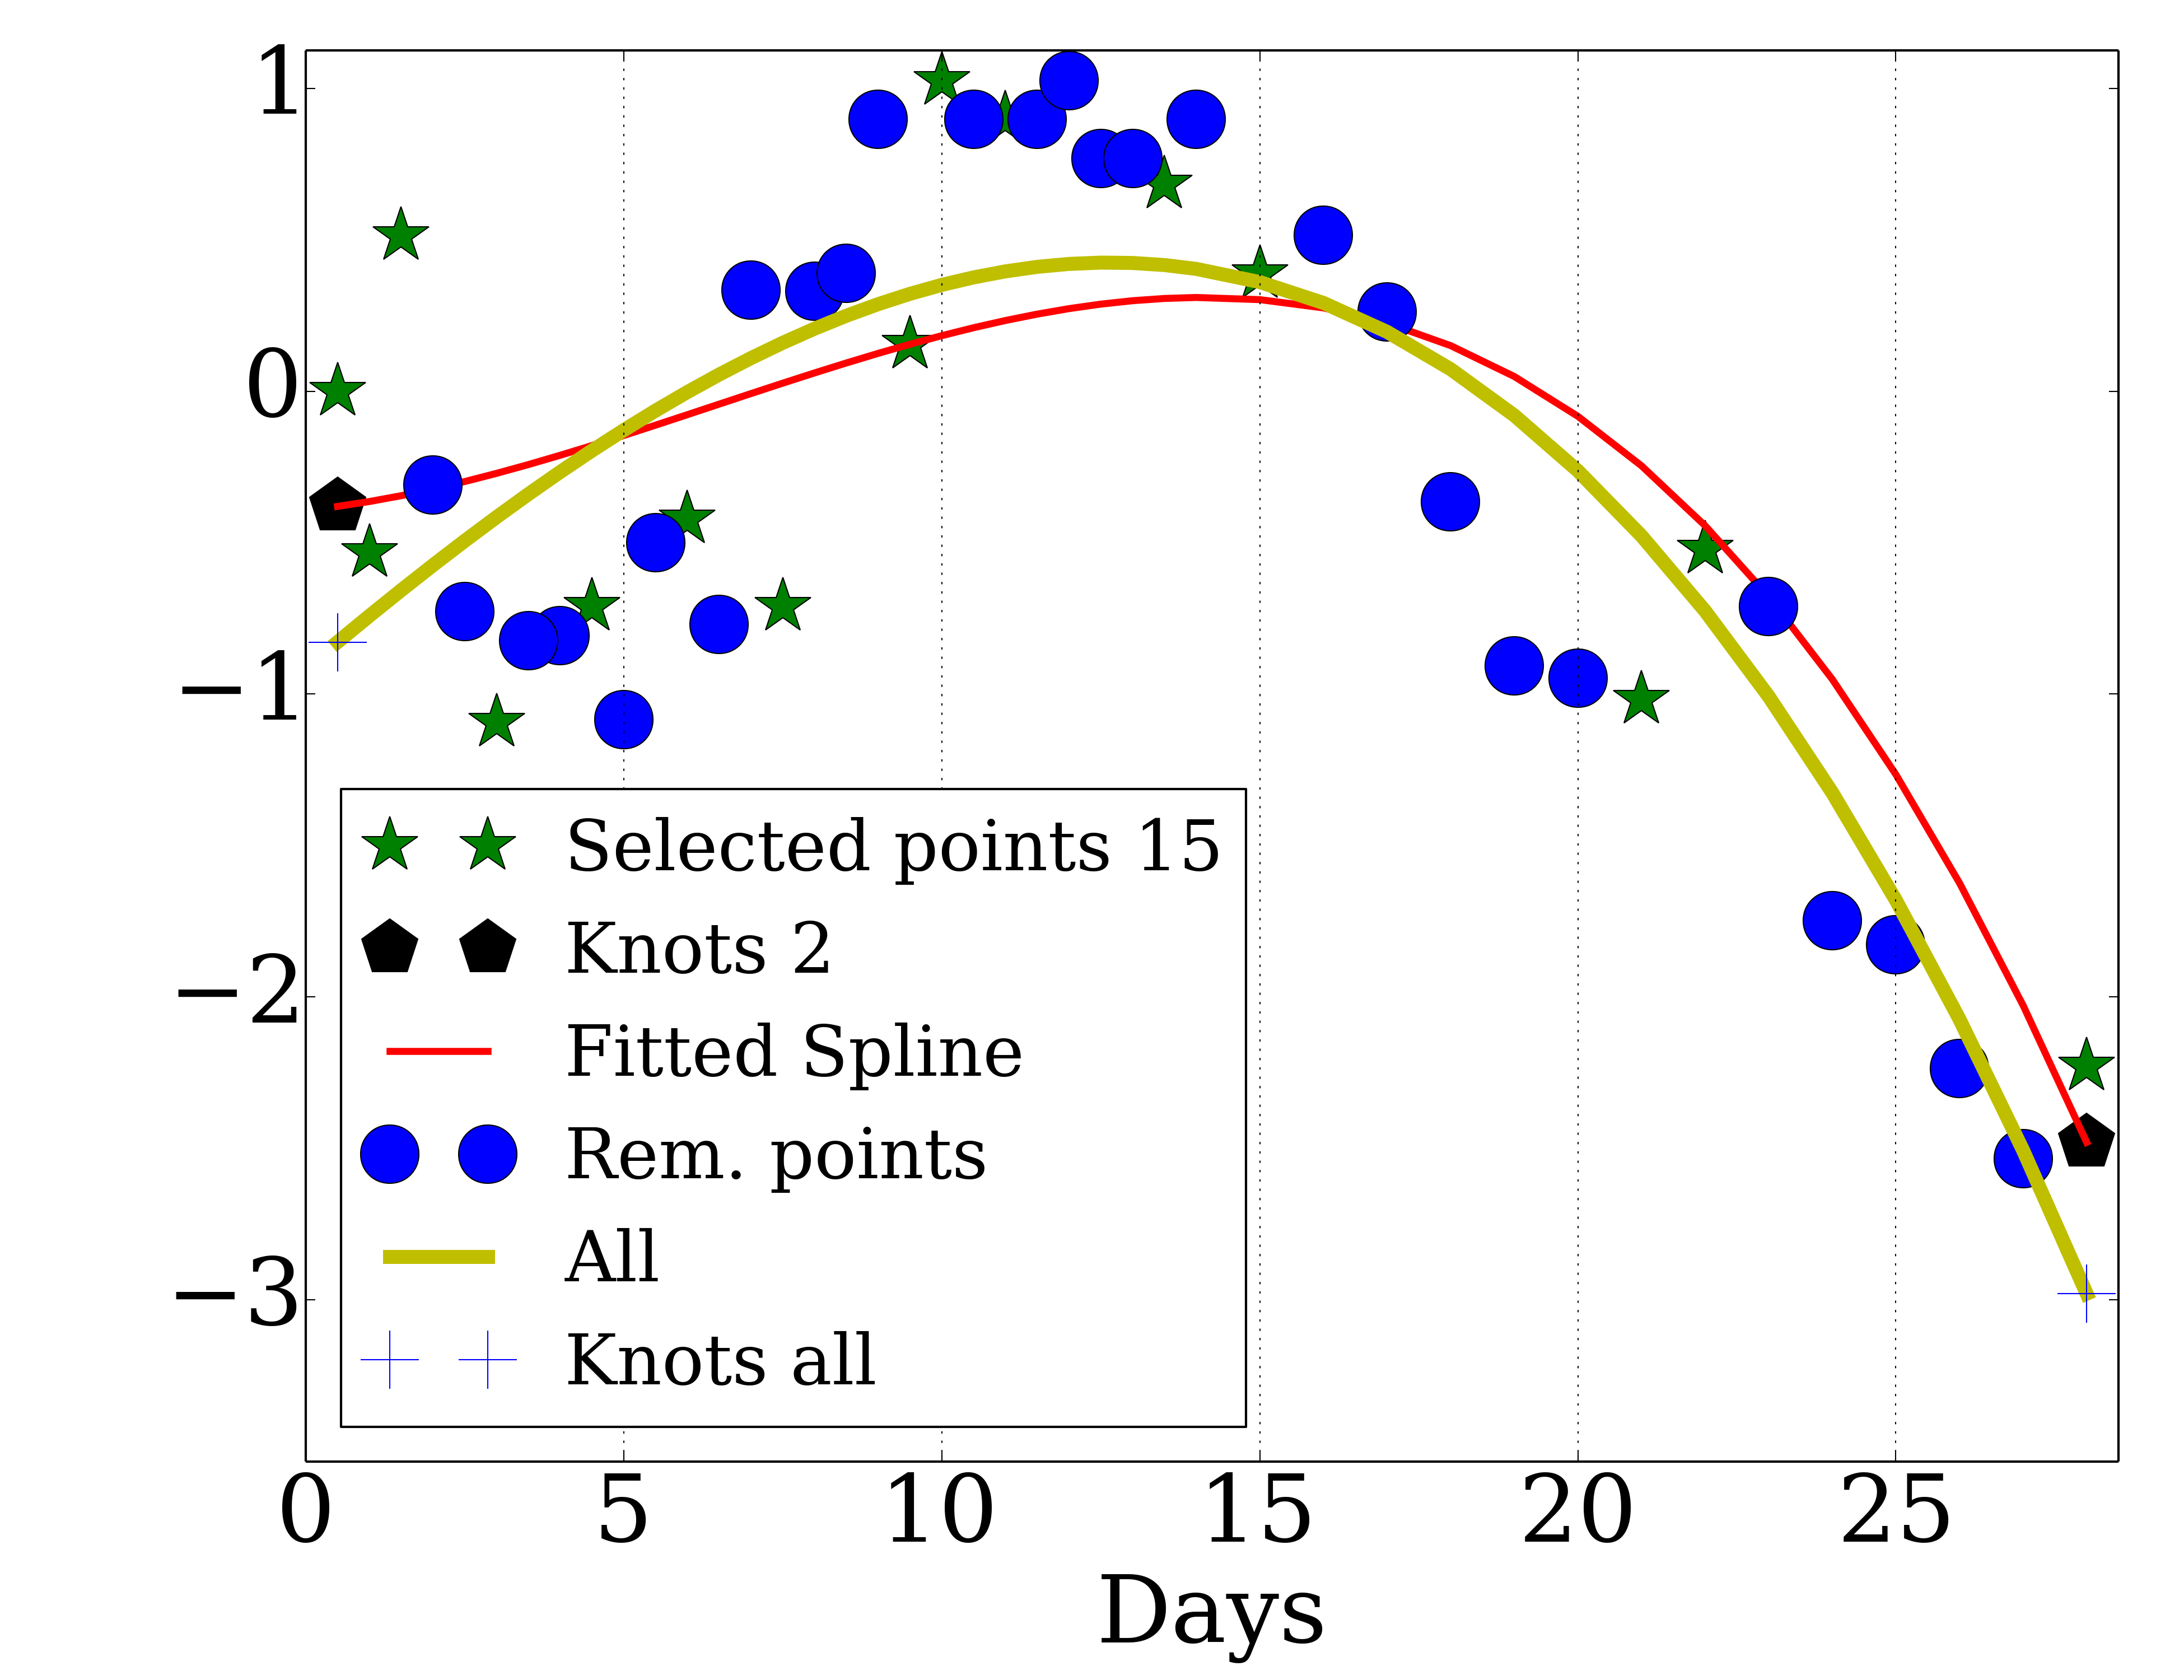
\includegraphics[scale=0.12]{{../newdata/splineplots15/Eln_15_all}.png}}
\\
\centering
\hfill
\subfloat[INMT]{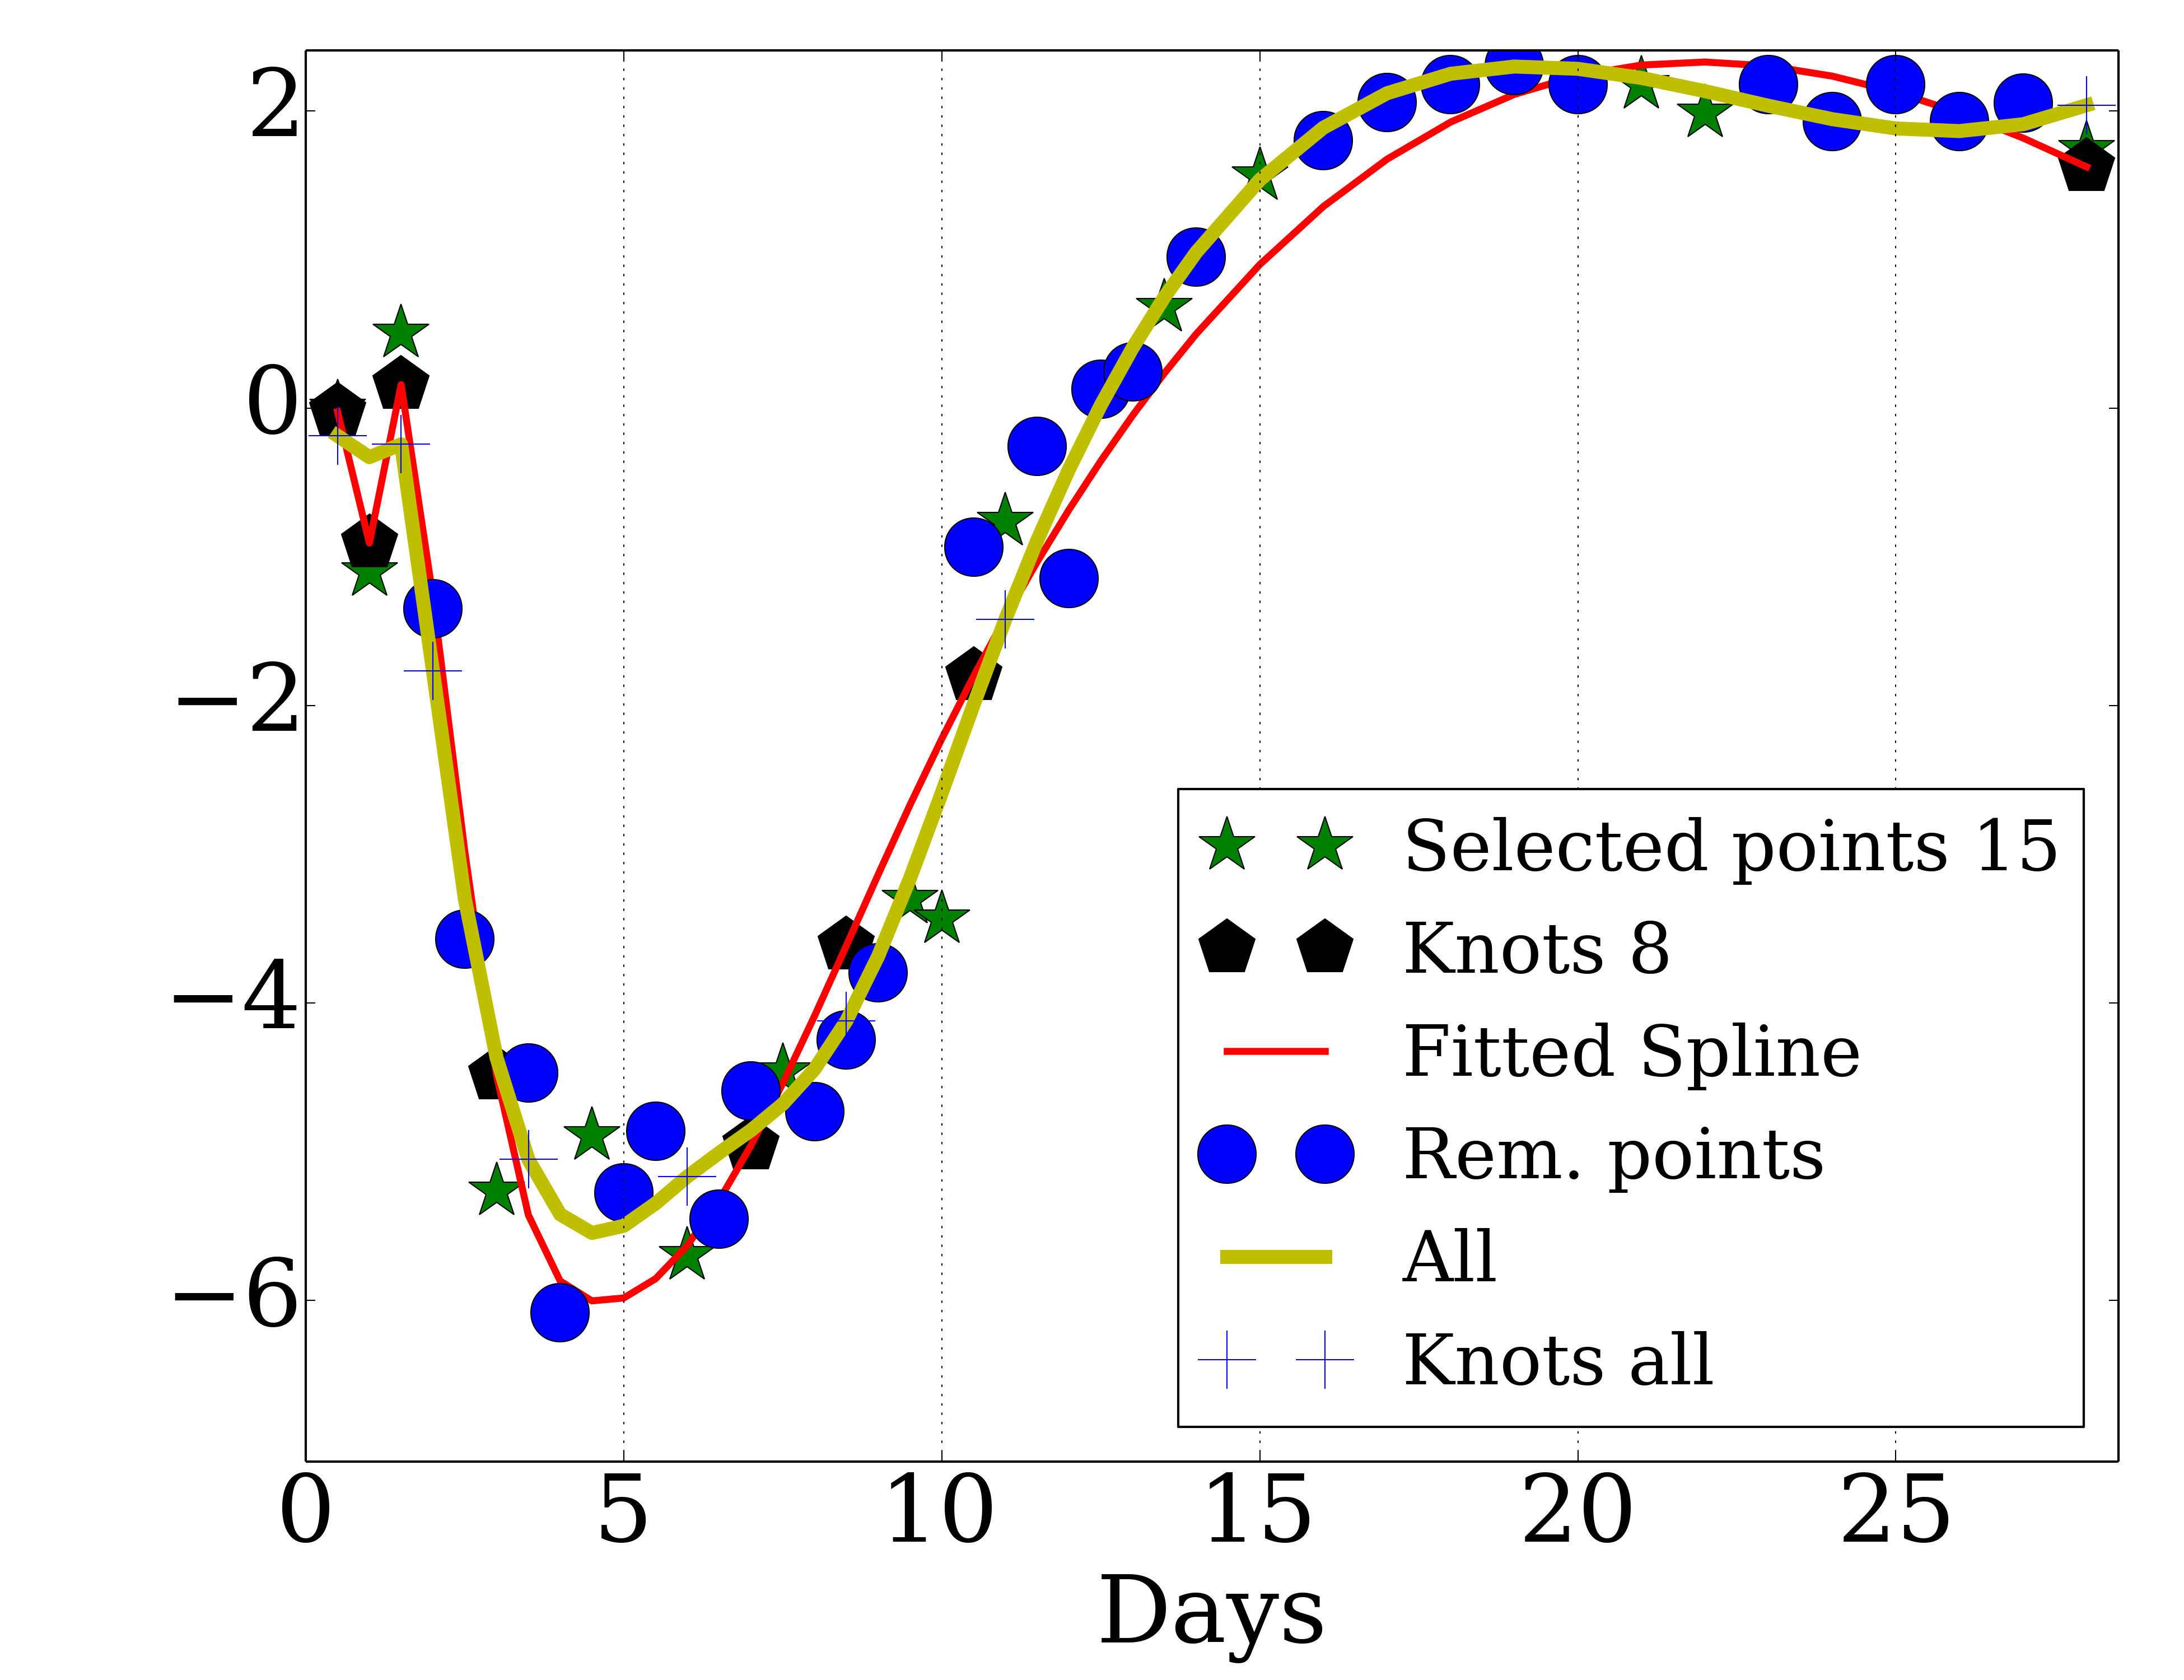
\includegraphics[scale=0.12]{{../newdata/splineplots15/INMT_15_all}.png}}
\hfill
\end{minipage}
\label{fig:centplots}
\end{figure}

\end{frame}


\begin{frame}
\frametitle{Spline vs Linear Error}

\begin{itemize}
\item Area difference is larger than $1.0$ for $102$ genes.
\end{itemize}

\begin{figure}[h]
\begin{minipage}{1.0\textwidth}
\subfloat[PDGFRA($8.3488$)]{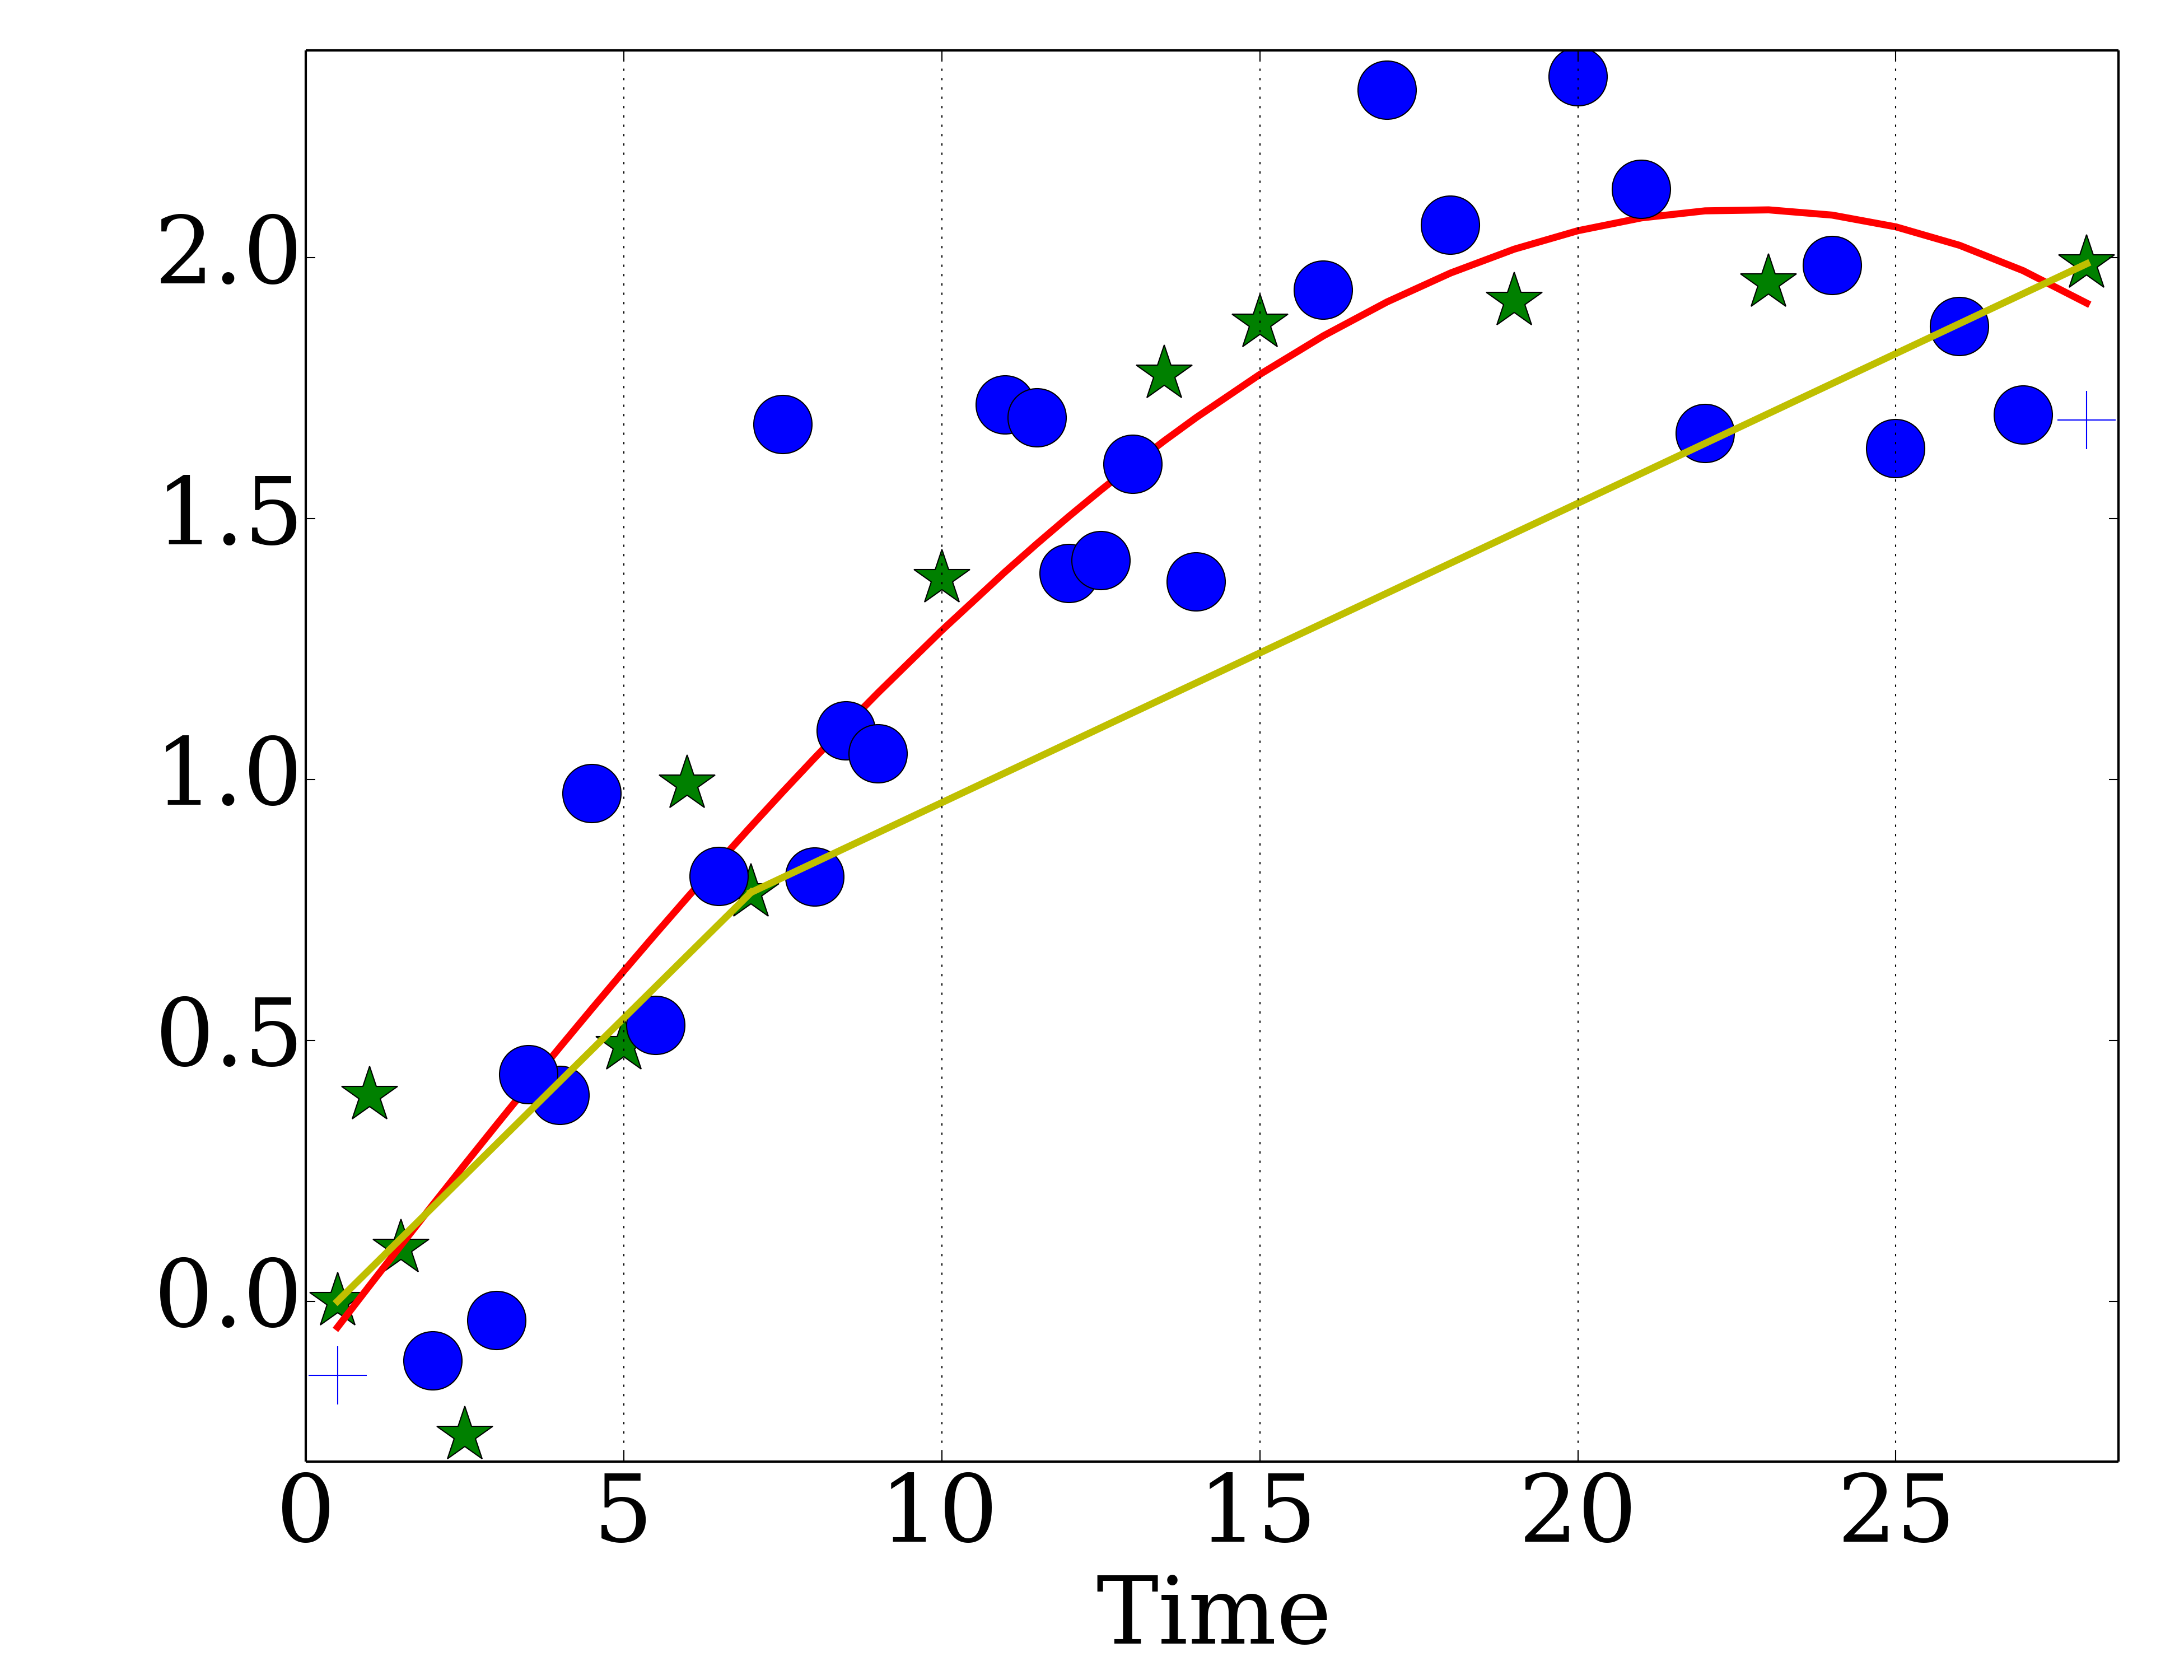
\includegraphics[scale=0.11]{{../newdata/17_PDGFRA13_all}.png}}
\hfill
\subfloat[ELN($9.5703$)]{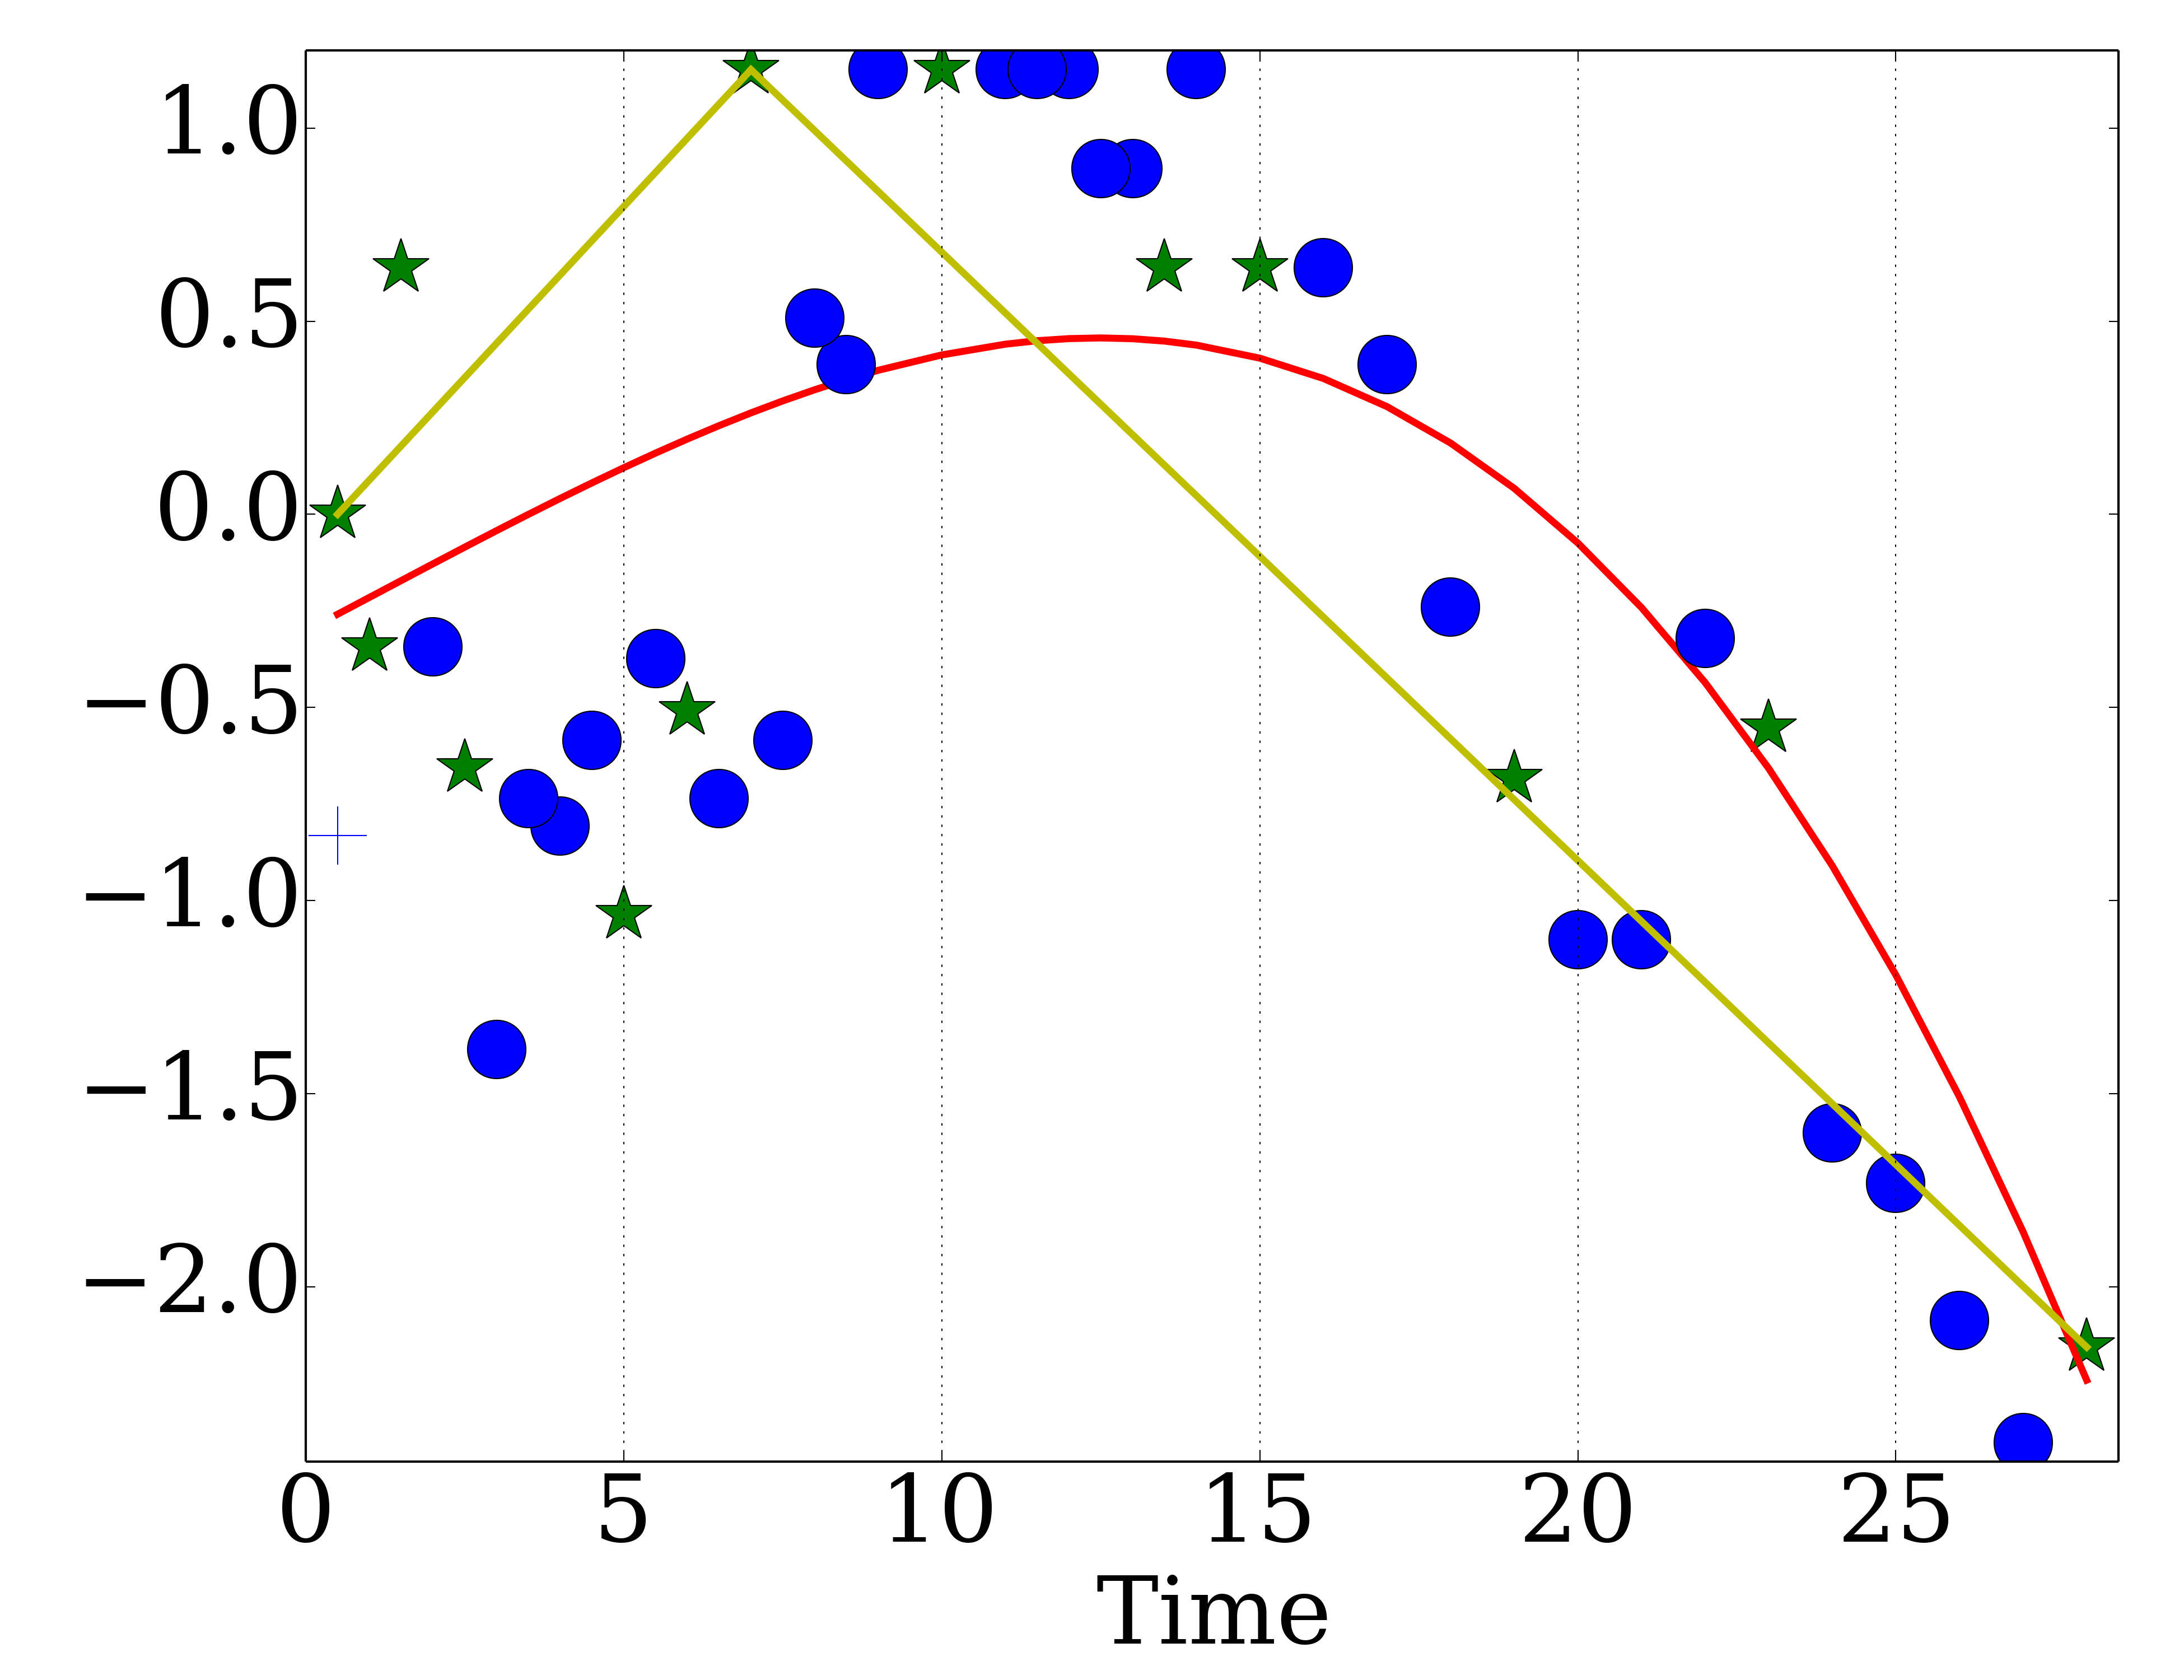
\includegraphics[scale=0.11]{{../newdata/splineAndLinear/14_Eln_13_all}.png}}
\\
\centering
\hfill
\subfloat[LRAT($25.24$)]{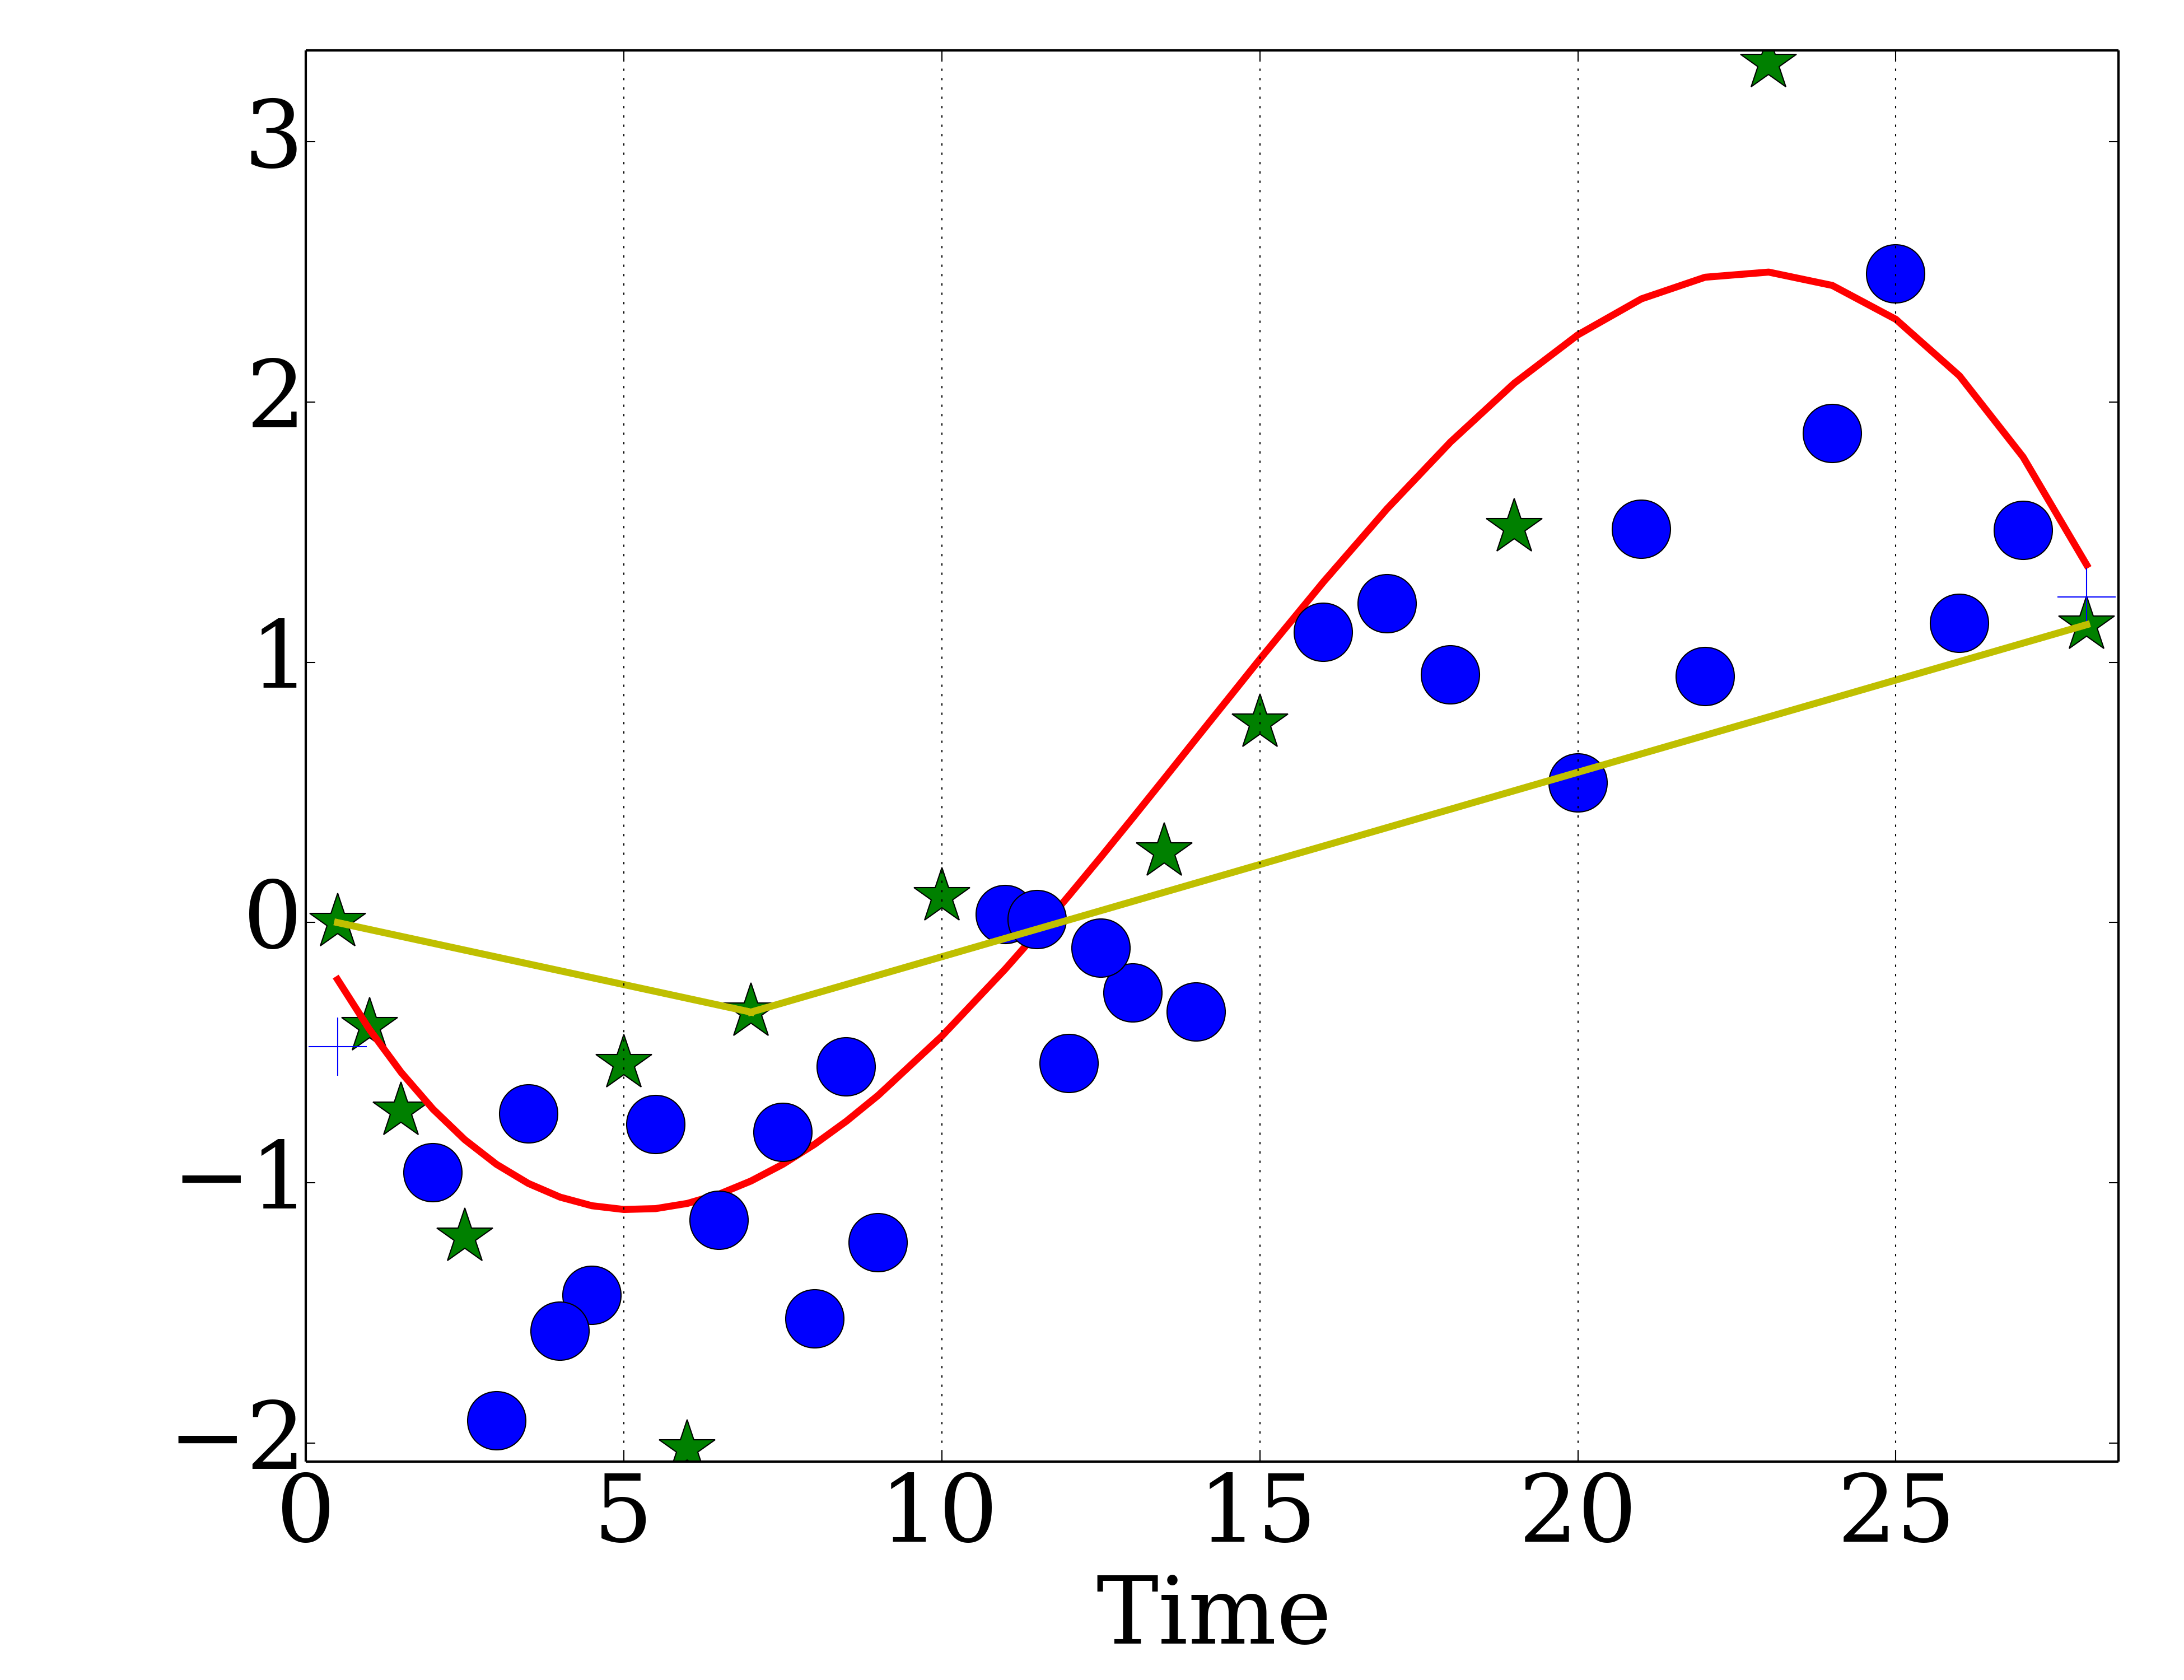
\includegraphics[scale=0.11]{{../newdata/splineAndLinear/1_LRAT_13_all}.png}}
\hfill
\end{minipage}
\label{fig:splinearplots}
\end{figure}

\end{frame}


\begin{frame}
\frametitle{Similarity of miRNA to mRNA}

\begin{itemize}
\item Using mRNA points gives $0.3312$ error for miRNA
\vspace{0.2cm}
\item Optimal points for miRNA are quite similar(error $0.3042$)
\[0.5, 1.0,1.5, 2.5, 4.0, 5.0, 7.0, 8.5, 10.0, 12.0, 15.0, 19.0, 23.0, 28.0\]

\end{itemize}

\end{frame}


\begin{frame}
\frametitle{Comparing miRNA and mRNA Errors}

\begin{itemize}
\item Error is decreasing by increasing number of selected points in both datasets
\end{itemize}

\begin{figure}[h]
\begin{minipage}{1.0\textwidth}
\subfloat[Performance analysis]{\includegraphics[scale=0.15]{{../mirnadata/perform}.png}}
\hfill
\subfloat[Remove $27.0$ and $28.0$]{\includegraphics[scale=0.15]{{../mirnadata/performRL2}.png}}
\end{minipage}
\label{fig:errplots}
\end{figure}

\end{frame}


\begin{frame}
\frametitle{miRNA Cluster Analysis}

\begin{itemize}
\item $8$ stable clusters
\vspace{0.1cm}
\item Clusters change more frequently than mRNA data.
\begin{itemize}
\item miRNA is noisier than mRNA data.
\end{itemize}
\end{itemize}

\begin{figure}[h]
\begin{minipage}{1.0\textwidth}
\centering
\subfloat[$8$ stable clusters]{\includegraphics[scale=0.2]{{../mirnadata/centplot}.png}}
\end{minipage}
\label{fig:centplotsmirna}
\end{figure}

\end{frame}


\begin{frame}
\frametitle{Detailed Analysis of miRNA Genes}

\begin{itemize}
\item Spline reconstruction performs better than linear one similar to mRNA dataset.
\end{itemize}

\begin{figure}[h]
\begin{minipage}{1.0\textwidth}
\subfloat[mmu-miR-100]{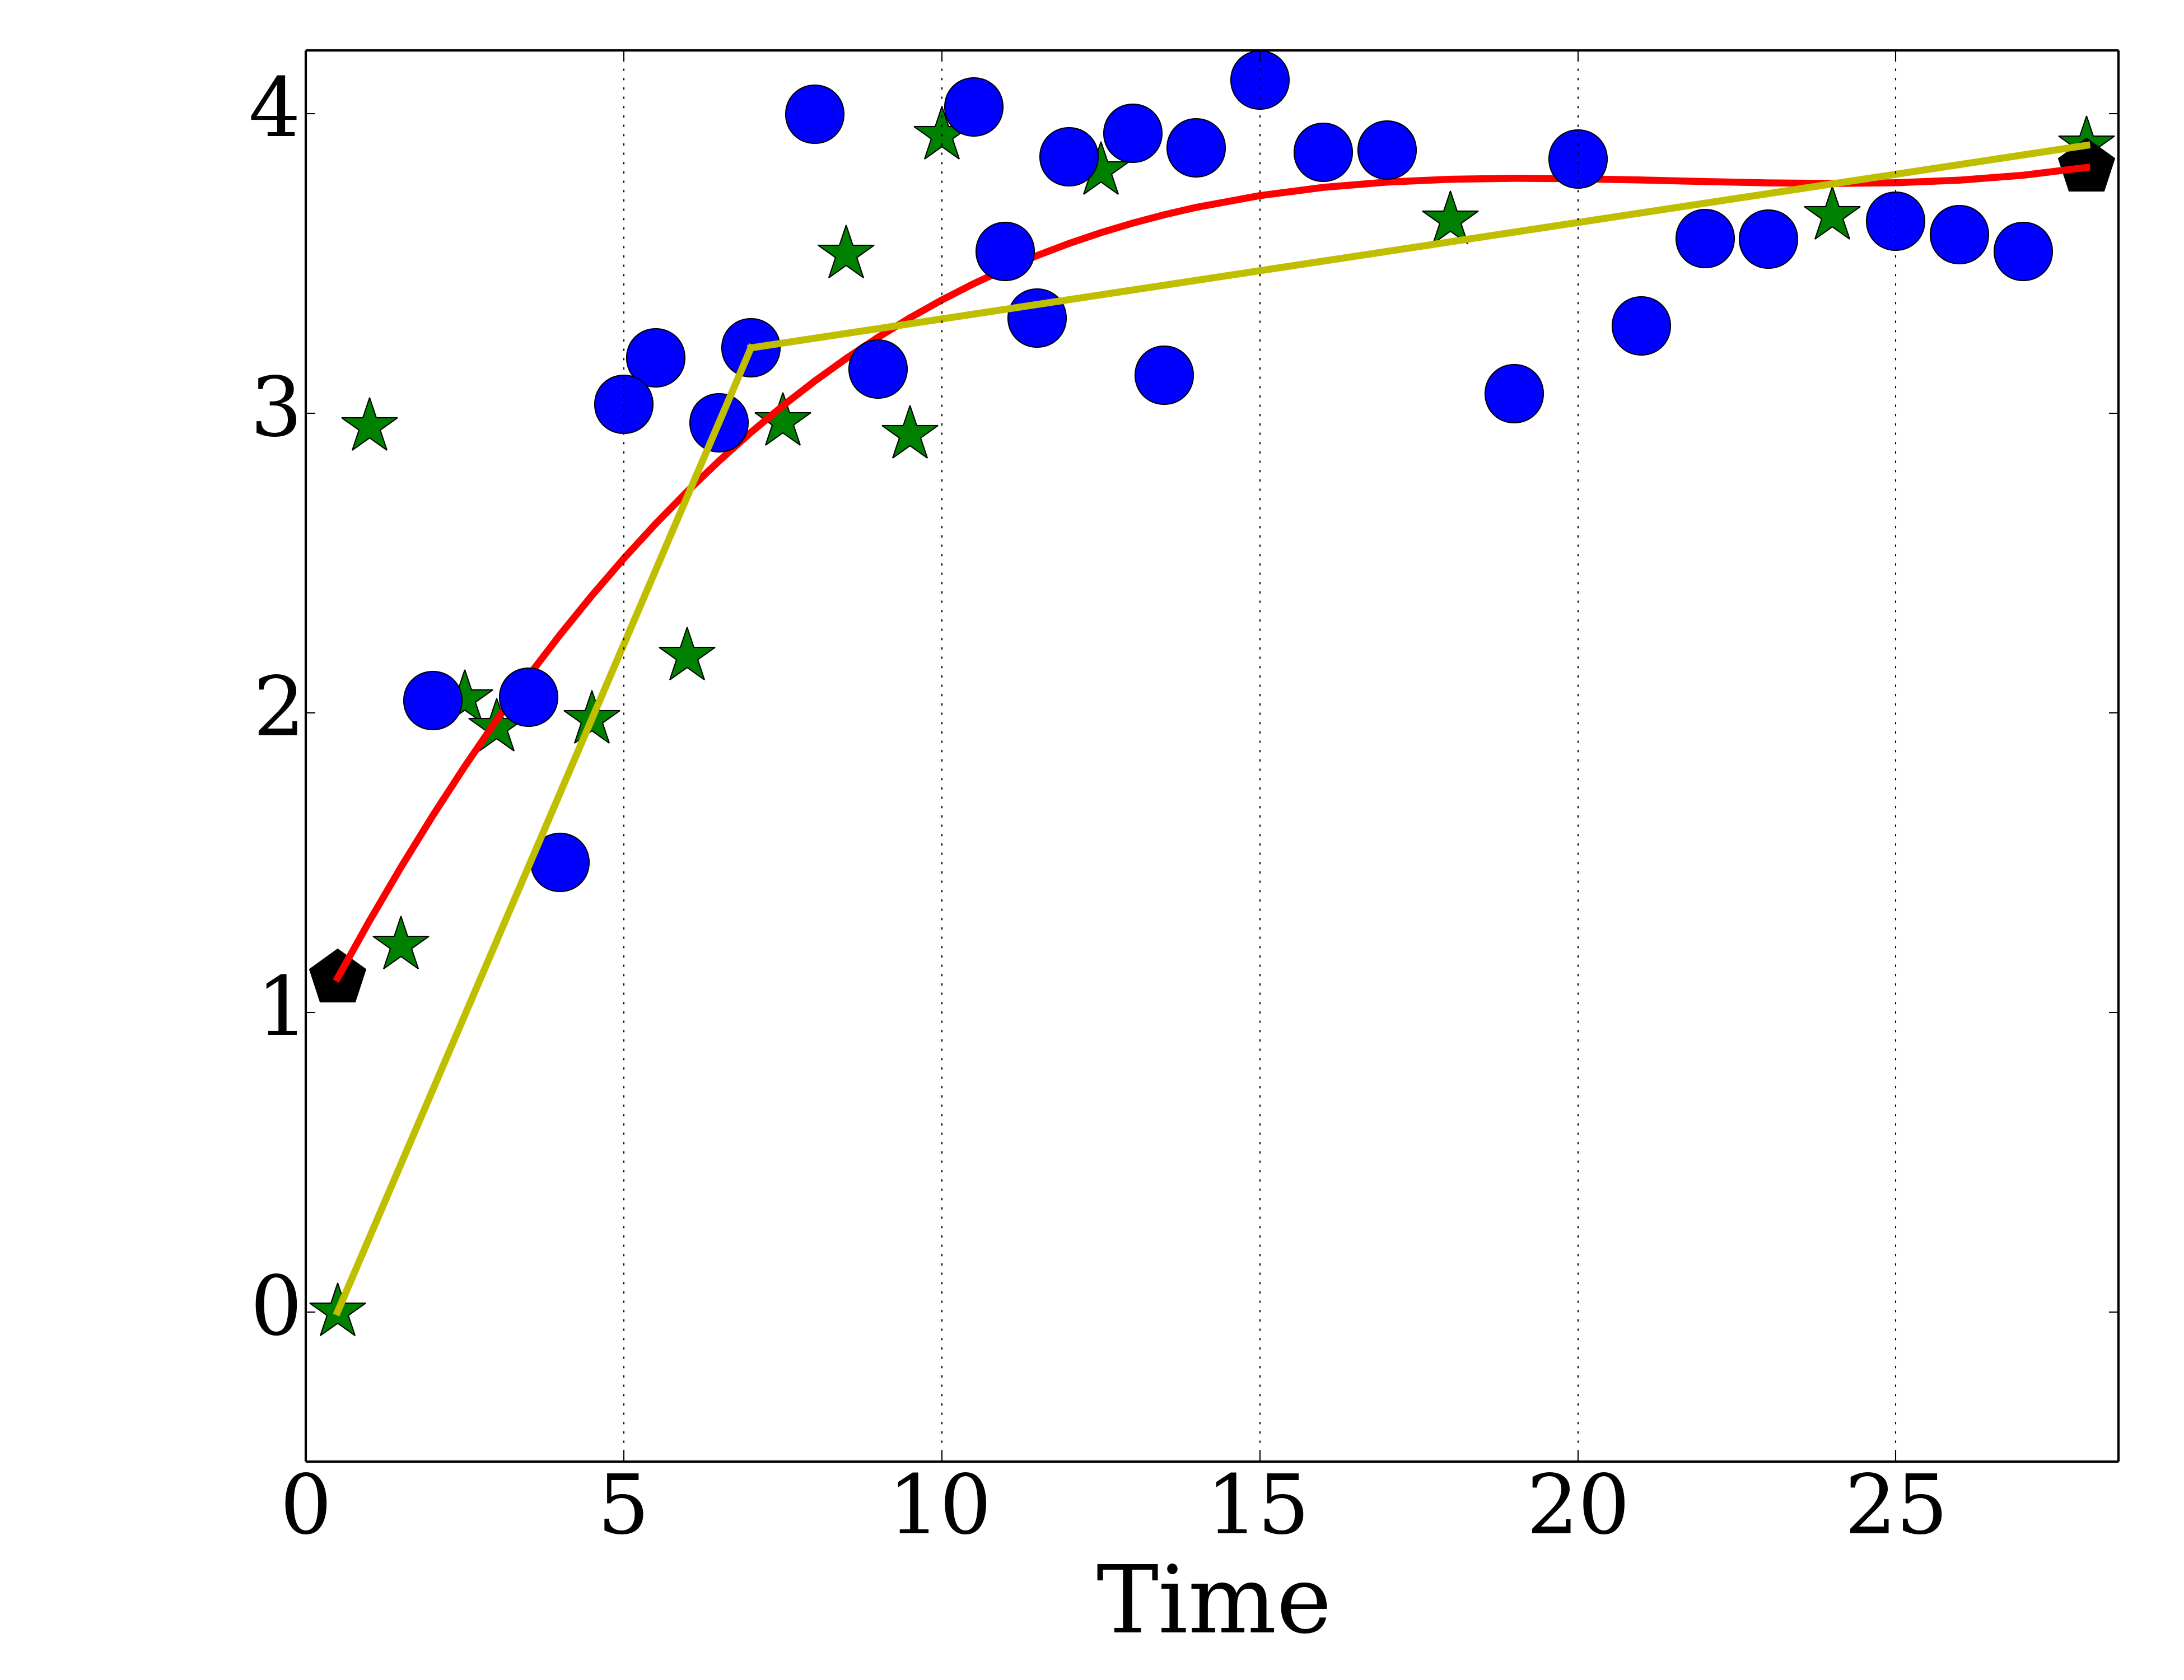
\includegraphics[scale=0.11]{{../mirnadata/splineplots15/uni/mmu-miR-100_15}.png}}
\hfill
\subfloat[mmu-miR-124]{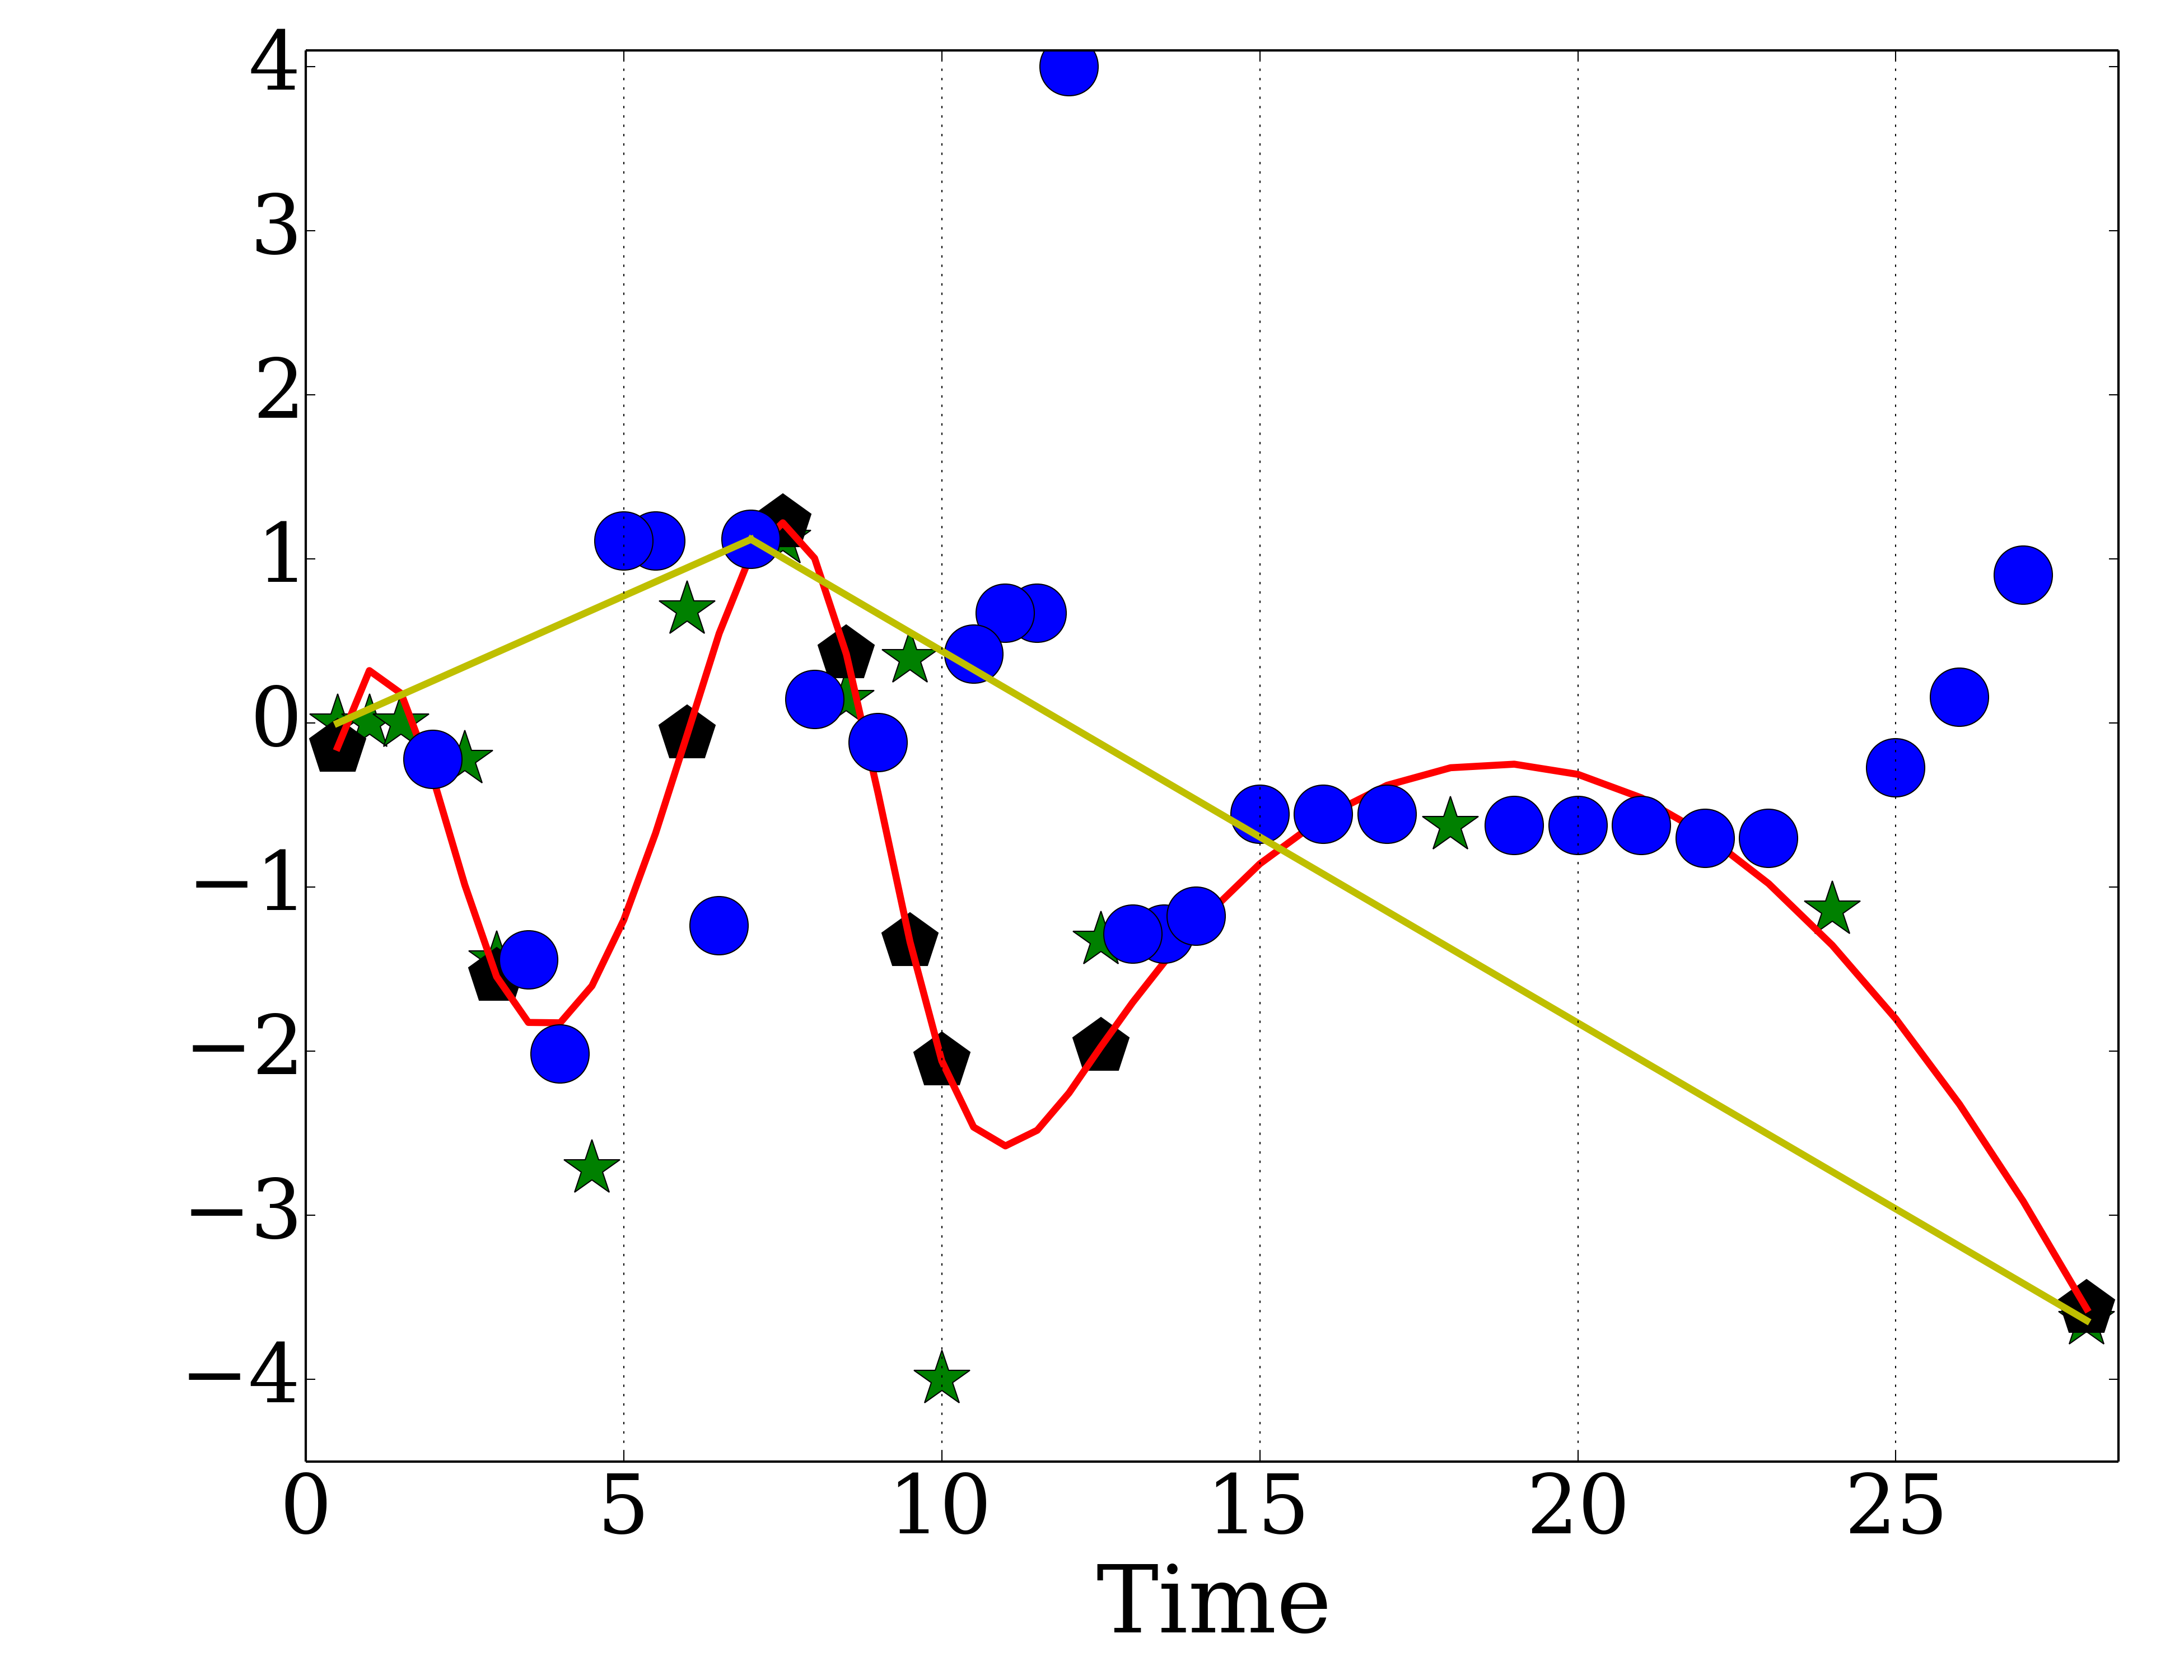
\includegraphics[scale=0.11]{{../mirnadata/splineplots15/uni/mmu-miR-124_15}.png}}
\\
\centering
\hfill
\subfloat[mmu-miR-377]{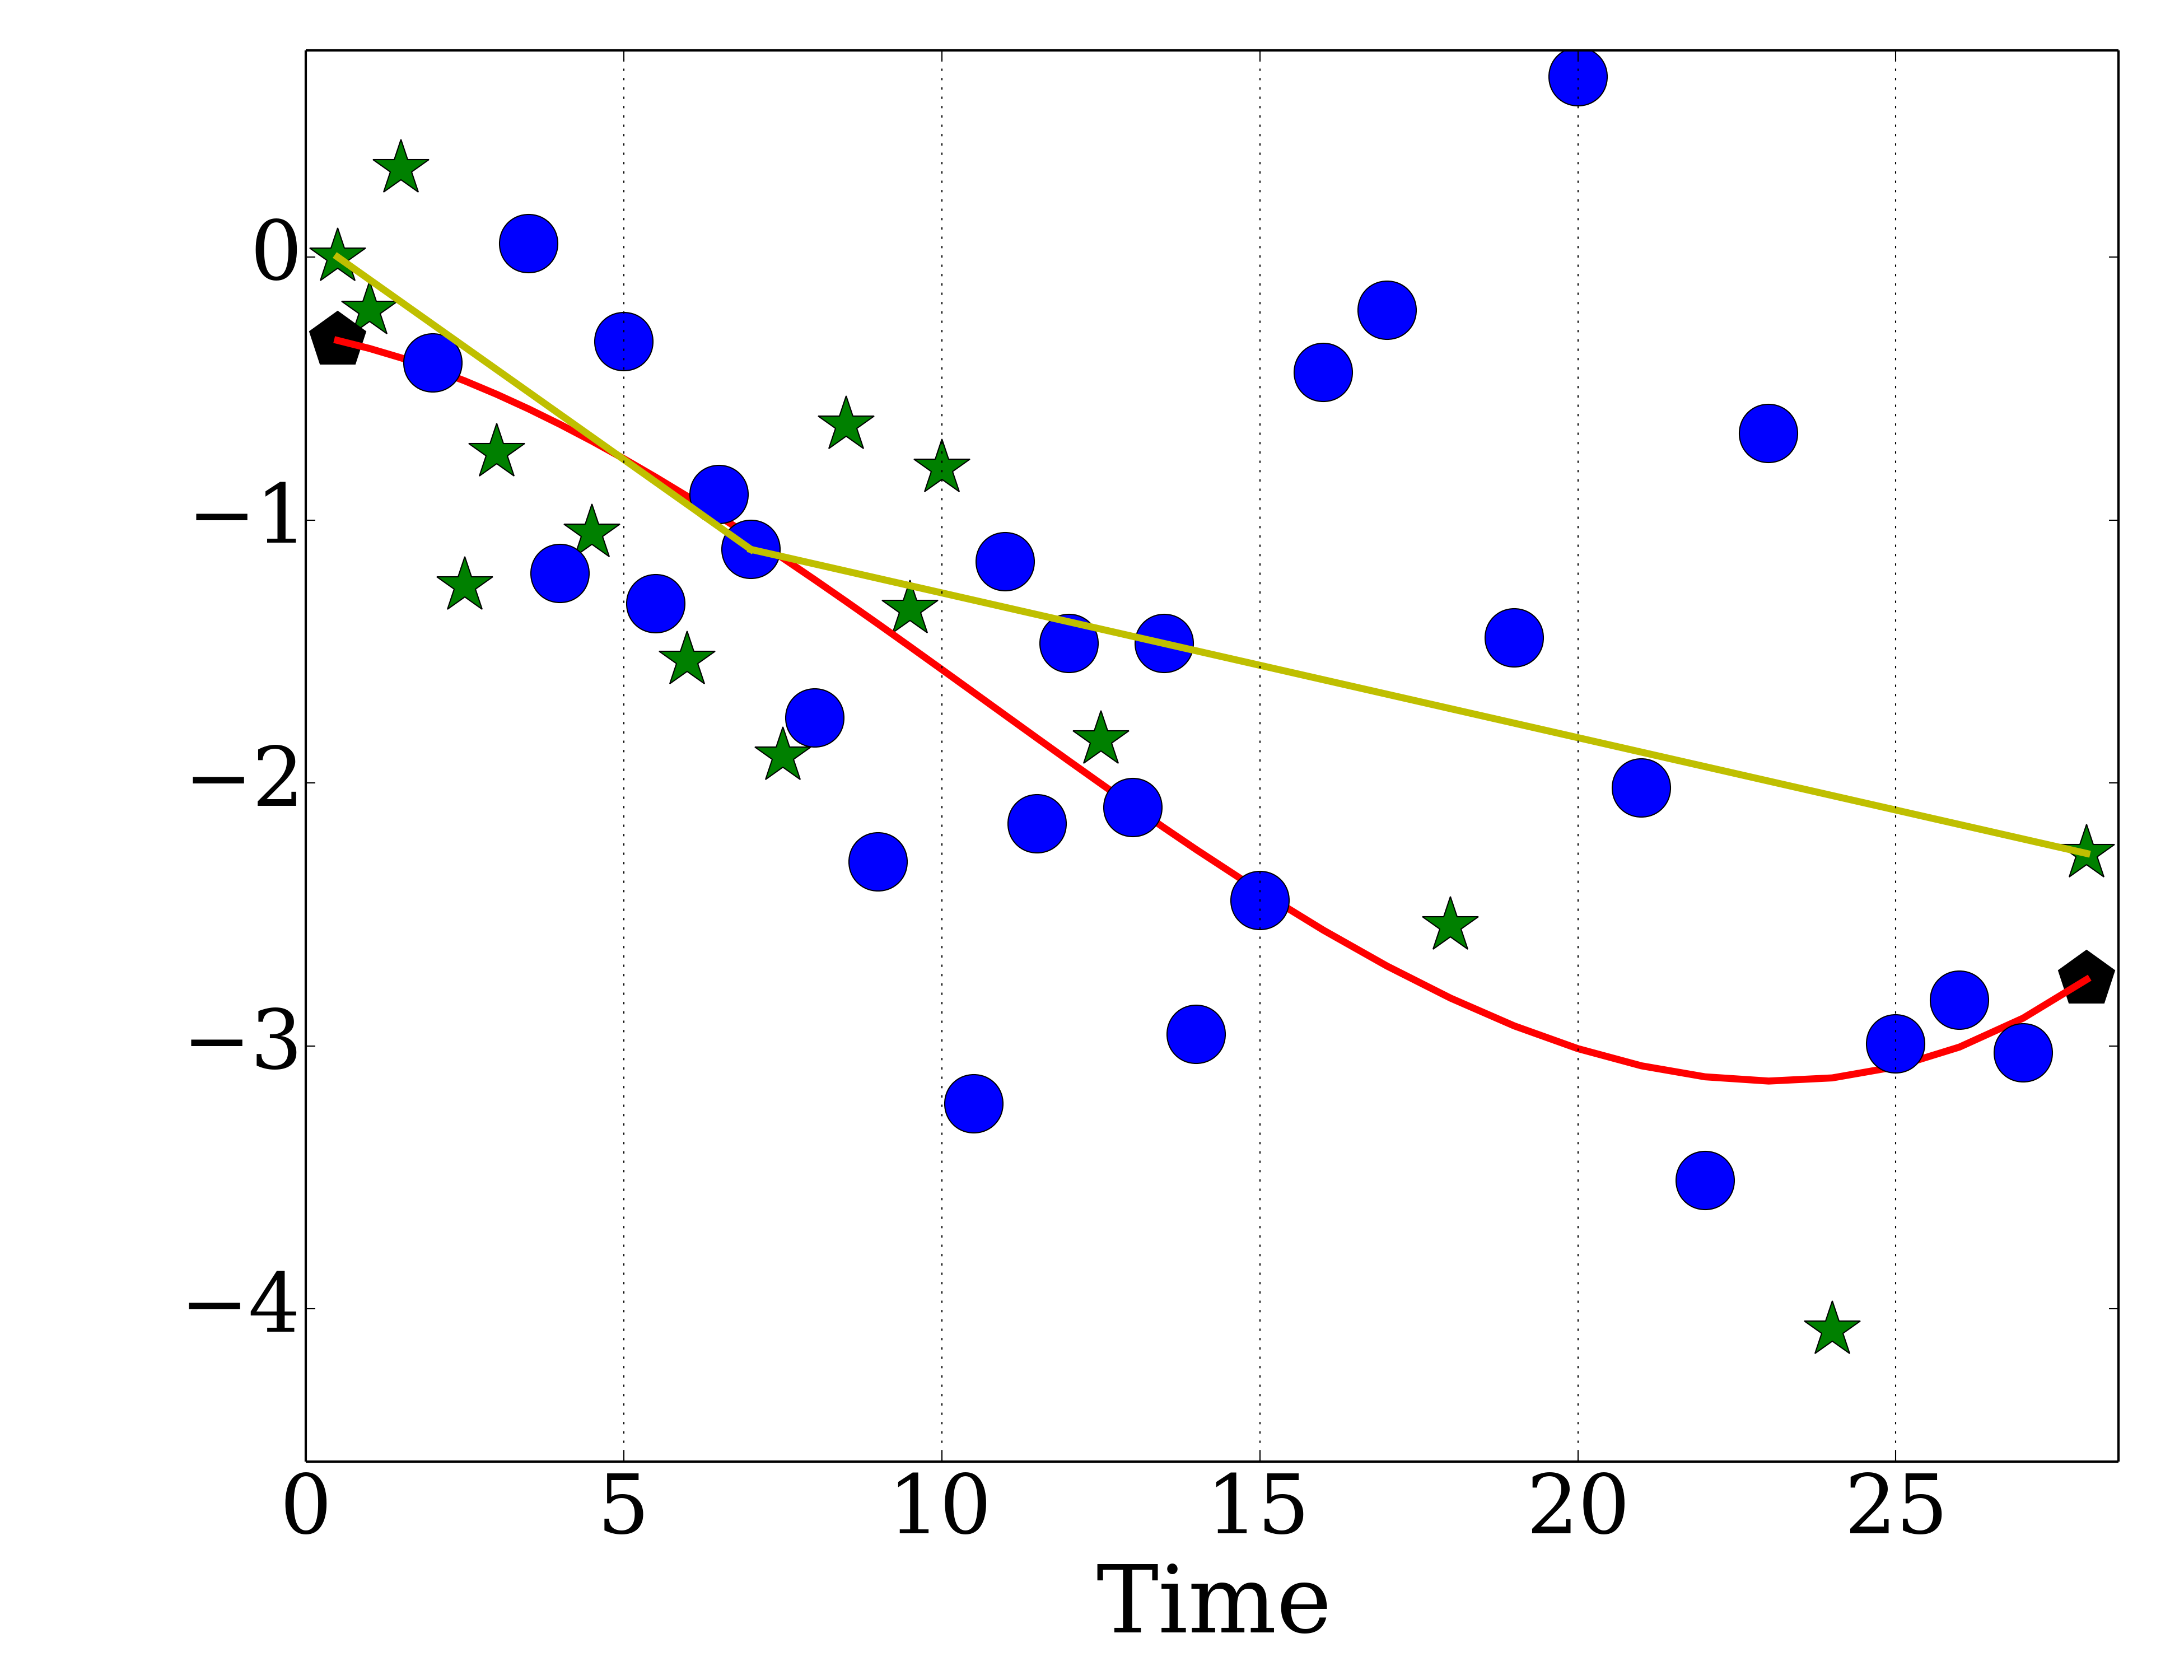
\includegraphics[scale=0.11]{{../mirnadata/splineplots15/uni/mmu-miR-377_15}.png}}
\hfill
\end{minipage}
\label{fig:mirnaplots}
\end{figure}

\end{frame}


\begin{frame}
\frametitle{Conclusion}

\begin{itemize}
\item Carefully selected subset of time points is important in
  reconstructing whole gene-expression over time
\vspace{0.1cm}
\item Spline based reconstruction outperforms simpler linear reconstruction
\vspace{0.1cm}
\item Analysis of mRNA is a nice representative of larger miRNA study
\begin{itemize}
\item Similar subset of time points can reconstruct both data
\end{itemize}
\end{itemize}

\end{frame}


\end{document}
